\apendice{Documentación de usuario}

\section{Introducción}

En este apartado se describirán los requisitos y directrices para que los nuevos usuarios sean capaces de entrar en la aplicación y usarla efectivamente.

\section{Requisitos de usuarios}

Para utilizar la aplicación, es esencial que el usuario tenga instalados en su ordenador Ganache y Expo. 
Por otro lado, el usuario debe de tener instalada la aplicación Expo Go en su teléfono móvil y es recomendable que el dispositivo este equipado con cámara, así como con sistemas de autenticación biométrica, como huella digital o reconocimiento facial. 
Además, es necesario que el teléfono móvil esté conectado a la misma red que el ordenador donde se ejecutan Ganache y Expo.

\section{Instalación}

El proceso de instalación del proyecto se detalla en la sección \ref{sec:instalacionProyecto}. 
Se puede resumir en:

\begin{enumerate}

\item Clonar el repositorio.

\item Ir al archivo \textbf{Code/AppContractMe/src/ContractConexion/EtherProvider.js} y sustituir la variable `Url' por la IP de tu ordenador.

\item Desde el directorio \textbf{Code/AppContractMe} ejecutar \textbf{npx expo install} para descargar todas las dependencias.

\item ejecutar el comando \textbf{ganache --host \textit{tu\_ip} } desde cualquier lado en la terminal.

\item Desde el directorio \textbf{Code/AppContractMe} ejecutar \texttt{npx expo start}

\item Asegurándose de que nos encontremos en la opción `Expo Go', desde la aplicación Expo en tu teléfono móvil escanear el código QR.

\end{enumerate}

\section{Manual del usuario}

A continuación se procede a ilustrar las funcionalidades básicas de la aplicación. Es destacable comentar que para poder interactuar con todas la funcionalidades de la aplicación serán necesario dos cuentas, una que ejerza como empleador y otra que ejerza como trabajador. Por lo que será necesario cerrar sesión y volver a abrirla con una cuenta diferente o usar dos dispositivos móviles simultáneamente.

\subsection{Identificación del usuario}

El primer paso para utilizar \textit{ContractMe}, es iniciar sesión para acceder a todas las funcionalidades de la misma. Es obligatorio rellenar tanto el campo de usuario (email) como el de la contraseña.
Ver imagen \ref{img:inicioSesion}.

\begin{figure}[h]
	\label{img:inicioSesion}
	\centering
	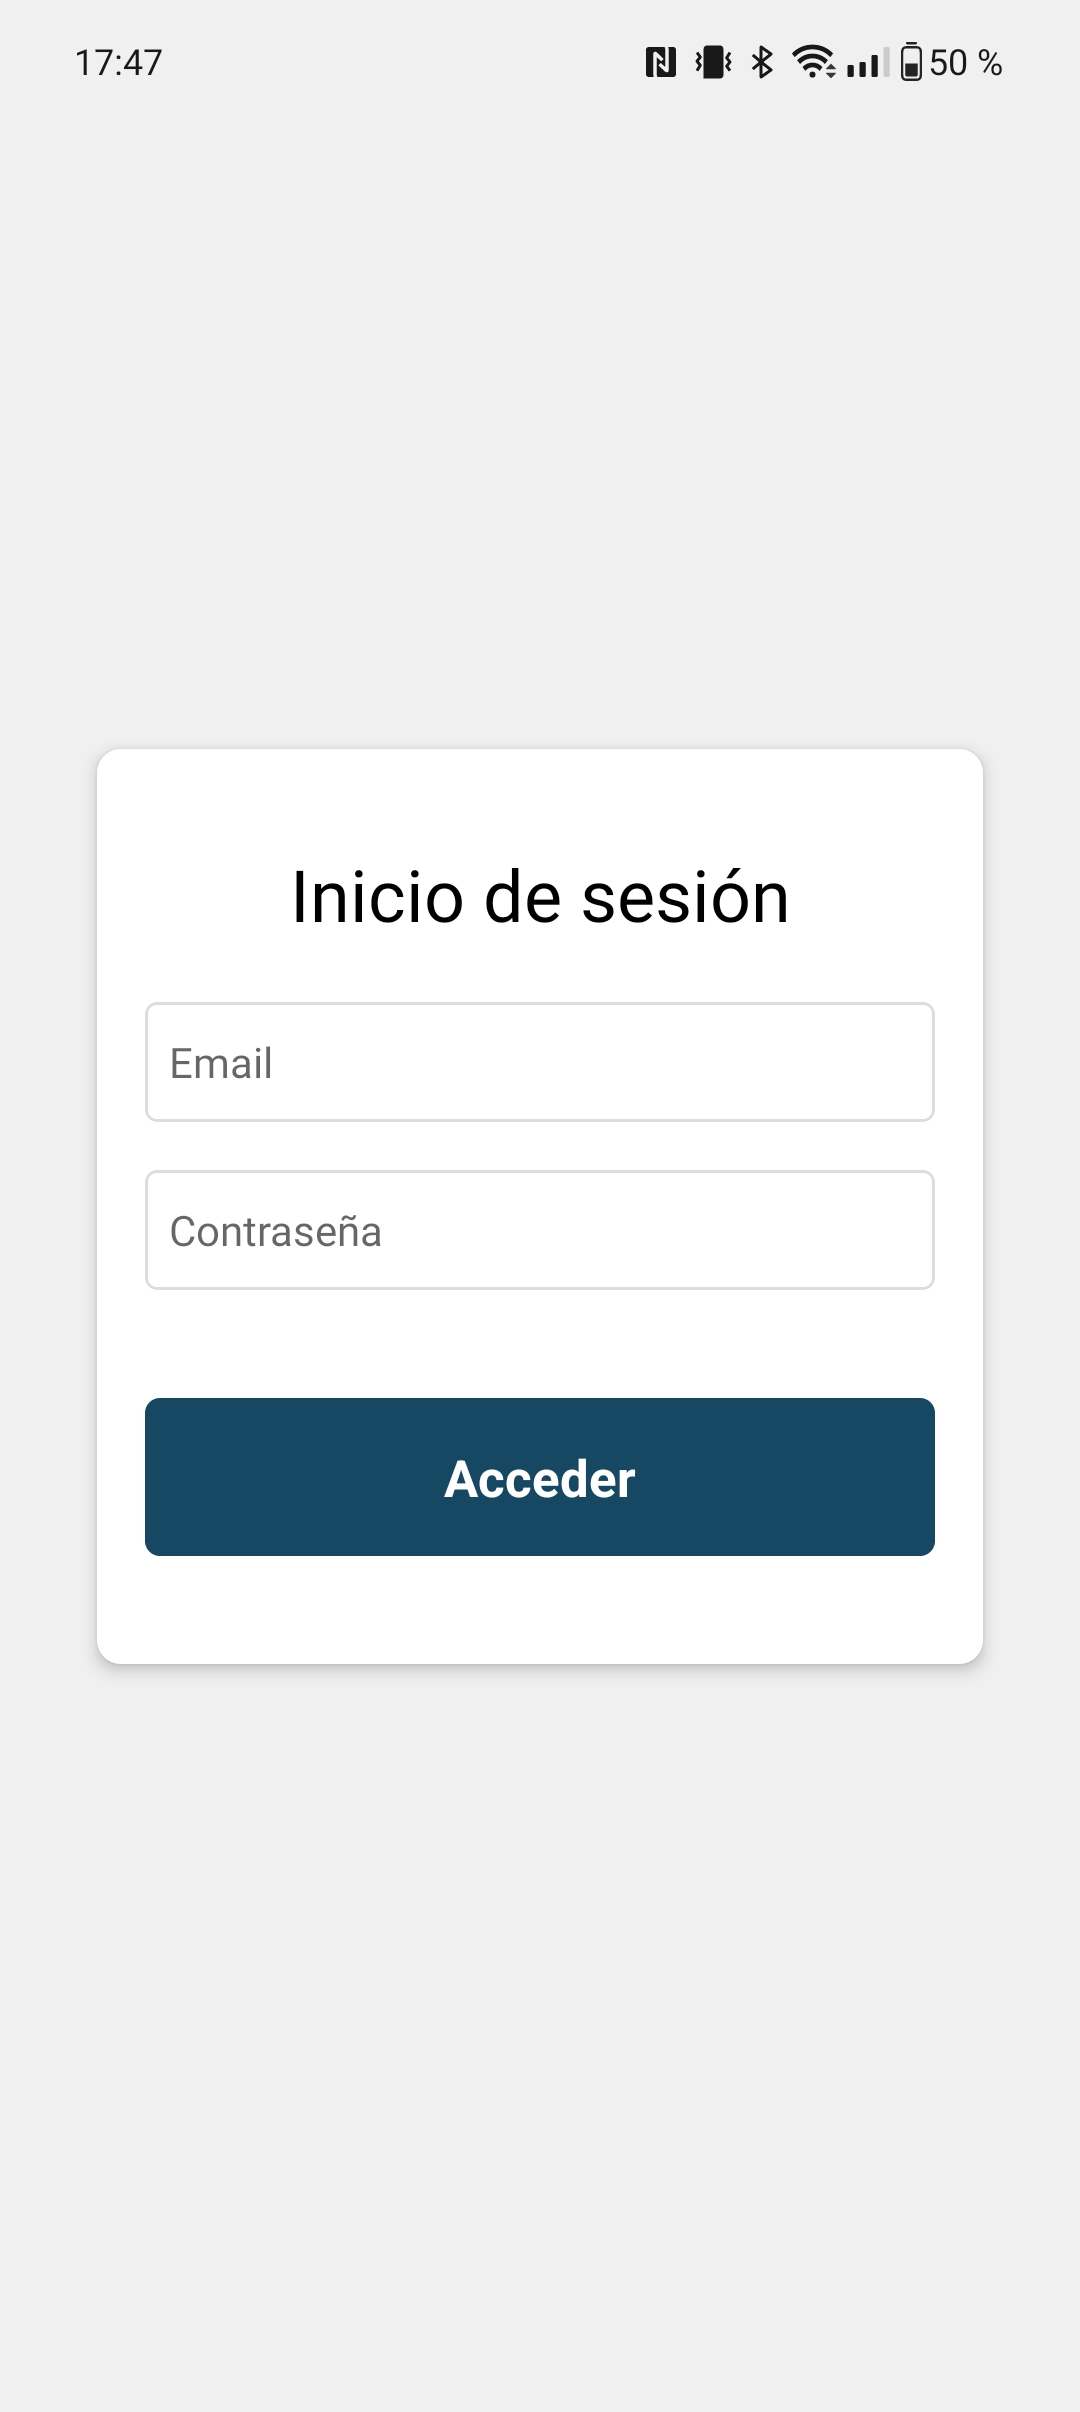
\includegraphics[width=0.40\textwidth]{inicioSesion}
	\caption[Pantalla inicio sesión]{Pantalla de inicio de sesión.}
\end{figure}

\subsection{Pantalla inicio}

Tras una identificación exitosa, todos los usuarios serán redirigidos a la pantalla inicial (imagen \ref{img:pantallaInicio}). Esta pantalla tiene los siguientes elementos:

\begin{itemize}

\item \textbf{Botón \textit{Crear Contrato}}: Al pulsar este botón se redigirá al usuario a una pantalla en la que mediante un formulario se podrá crear un contrato.

\item \textbf{Botón \textit{Firmar Contrato}}: Pulsando este botón se redirige al usuario a una pantalla donde aparecerán listados todos los contratos pendientes de firma que involucren al usuario.

\item \textbf{Botón \textit{Buscar Contratos}}: Este botón lleva al usuario a una pantalla donde puede buscar contratos que el empleador oferta dentro de la aplicación. 

\item \textbf{Botón \textit{Mis Contratos}}: Al pulsar este botón, el usuario es dirigido a una pantalla que lista todos los contratos en los que está involucrado, ya sea como dueño o como trabajador.
Los contratos pueden estar en distintos estados, bien activos o concluidos.

\end{itemize}

\begin{figure}[h]
	\label{img:pantallaInicio}
	\centering
	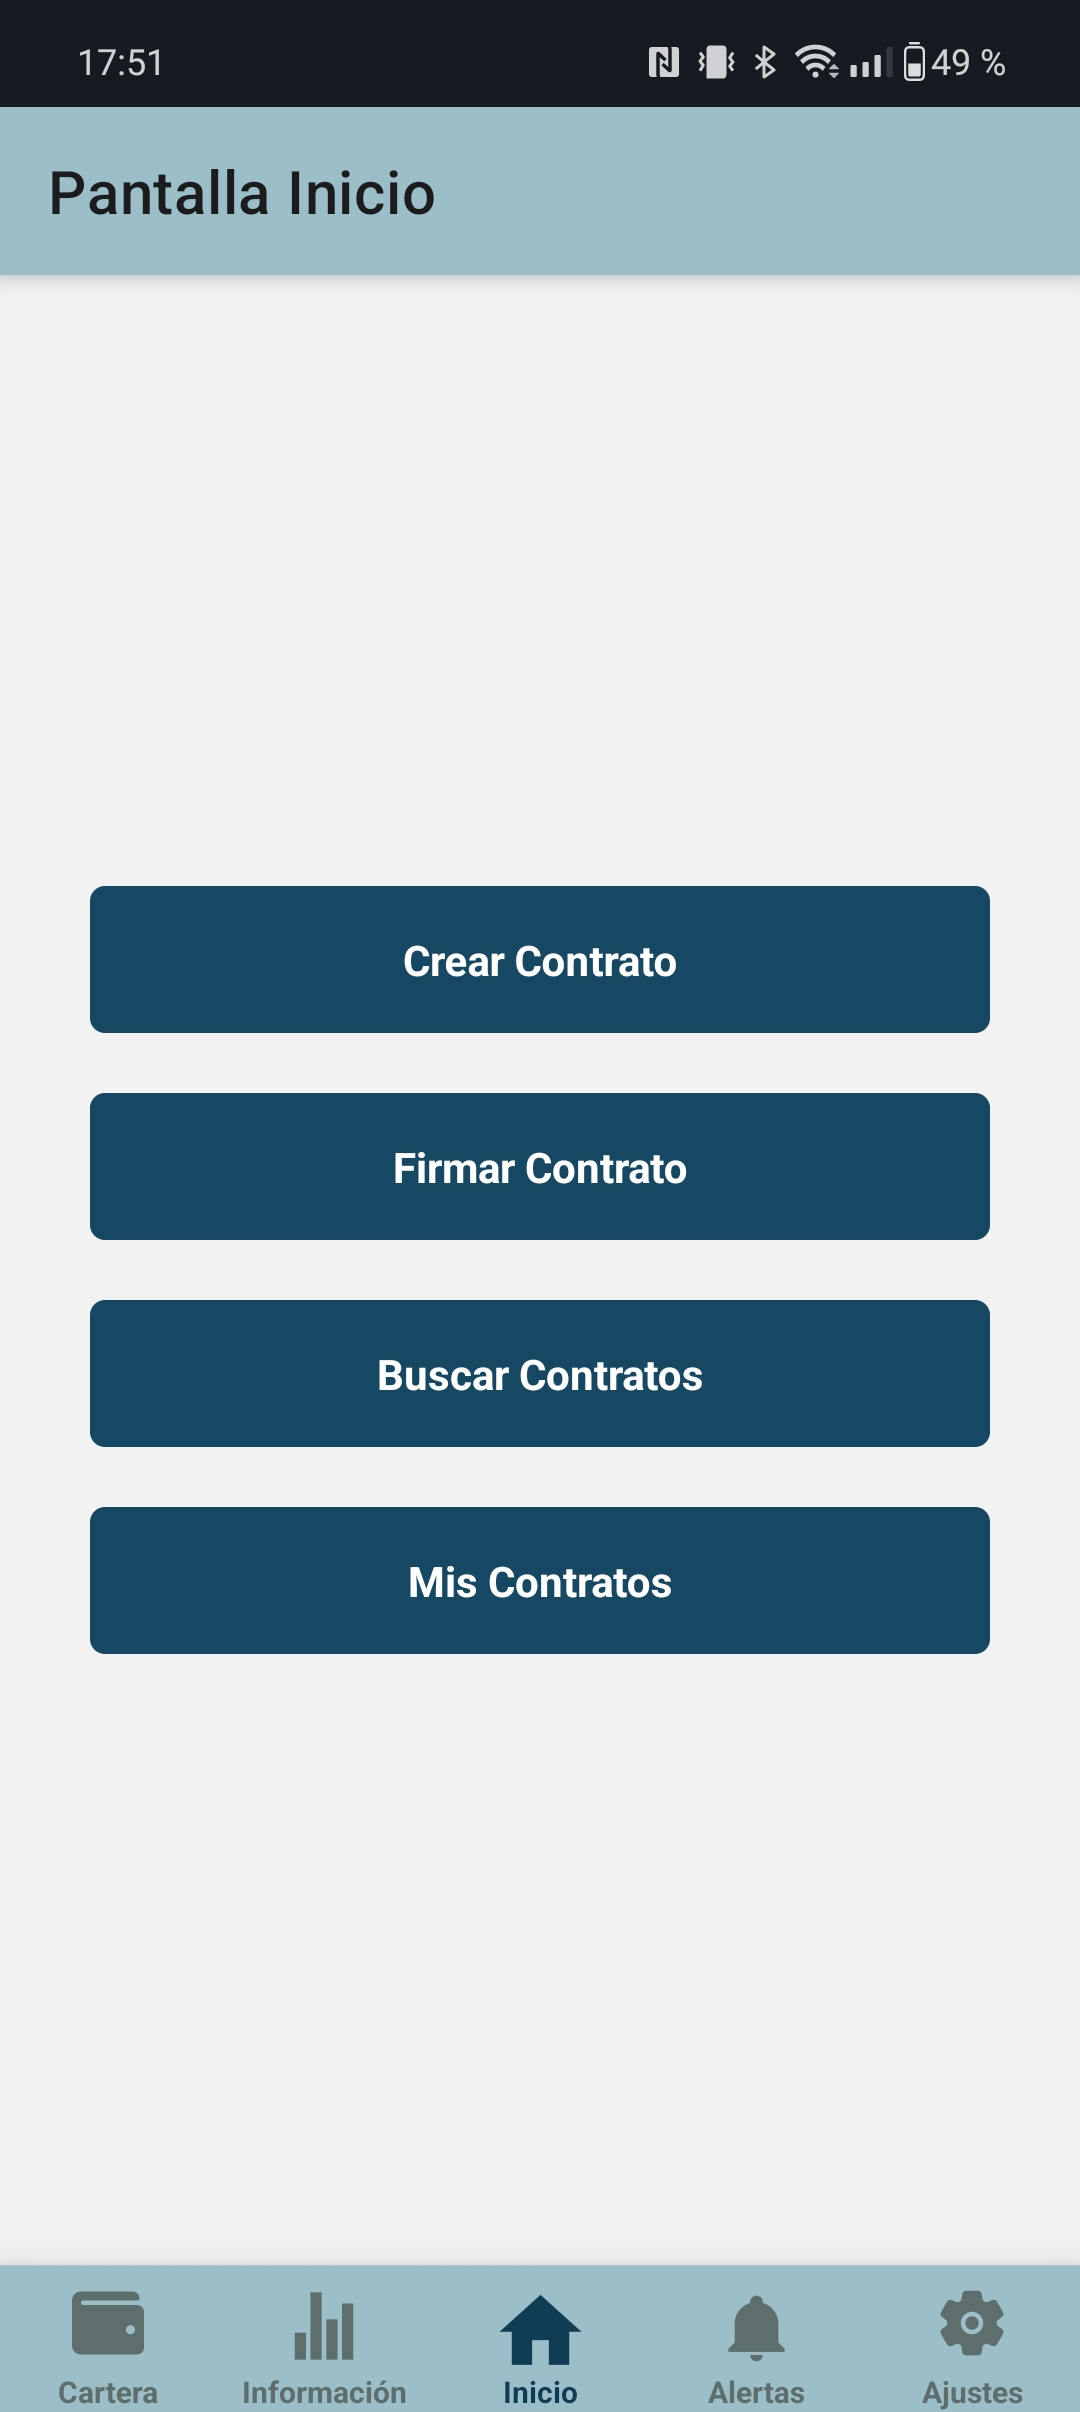
\includegraphics[width=0.40\textwidth]{pantallaInicio}
	\caption[Pantalla inicio]{Pantalla de inicio.}
\end{figure}


\subsection{Crear contrato}
\label{sec:CrearContrato}

Esta pantalla (ver imagen \ref{img:crearContrato}) muestra una interfaz destinada a la creación de un contrato laboral, cuenta con los siguientes campos:

\begin{itemize}

\item \textbf{Título del contrato}: En este campo se debe ingresar el título del contrato.

\item \textbf{Descripción del contrato}: Aquí se especifican los detalles del contrato. Este campo es importante para definir claramente las tareas y expectativas de la posición.

\item \textbf{Dirección del destinatario}: Este campo esta destinado para ingresar la dirección de la billetera del trabajador, la cual se usará tanto para identificar al trabajador como para ingresar el salario.
Cabe remarcar que este campo es opcional, y en el caso de no ser rellenado se considerará que se esta ofertando el trabajo y se mostrará a todos los usuarios de la aplicación para su firma.

\item \textbf{Salario del trabajador}: En este campo se debe introducir el salario del trabajador, especificado en Ethereum.

\item \textbf{Fecha inicio y fin}: Estos campos se utilizan para definir la duración del contrato, indicando cuándo comenzará y terminará. Al introducir los datos aparecerá un calendario y un reloj permitiendo seleccionar la hora exacta de inicio y fin del contrato.

\end{itemize}

Finalmente, usando el botón `crear contrato', si todos los datos han sido introducidos correctamente, aparecerá una ventana emergente que confirmará que el contrato ha sido creado.
En caso de querer retroceder, el usuario puede usar el botón de retroceso del móvil o cualquiera de los botones del menú de la aplicación.

\begin{figure}[h]
	\label{img:crearContrato}
	\centering
	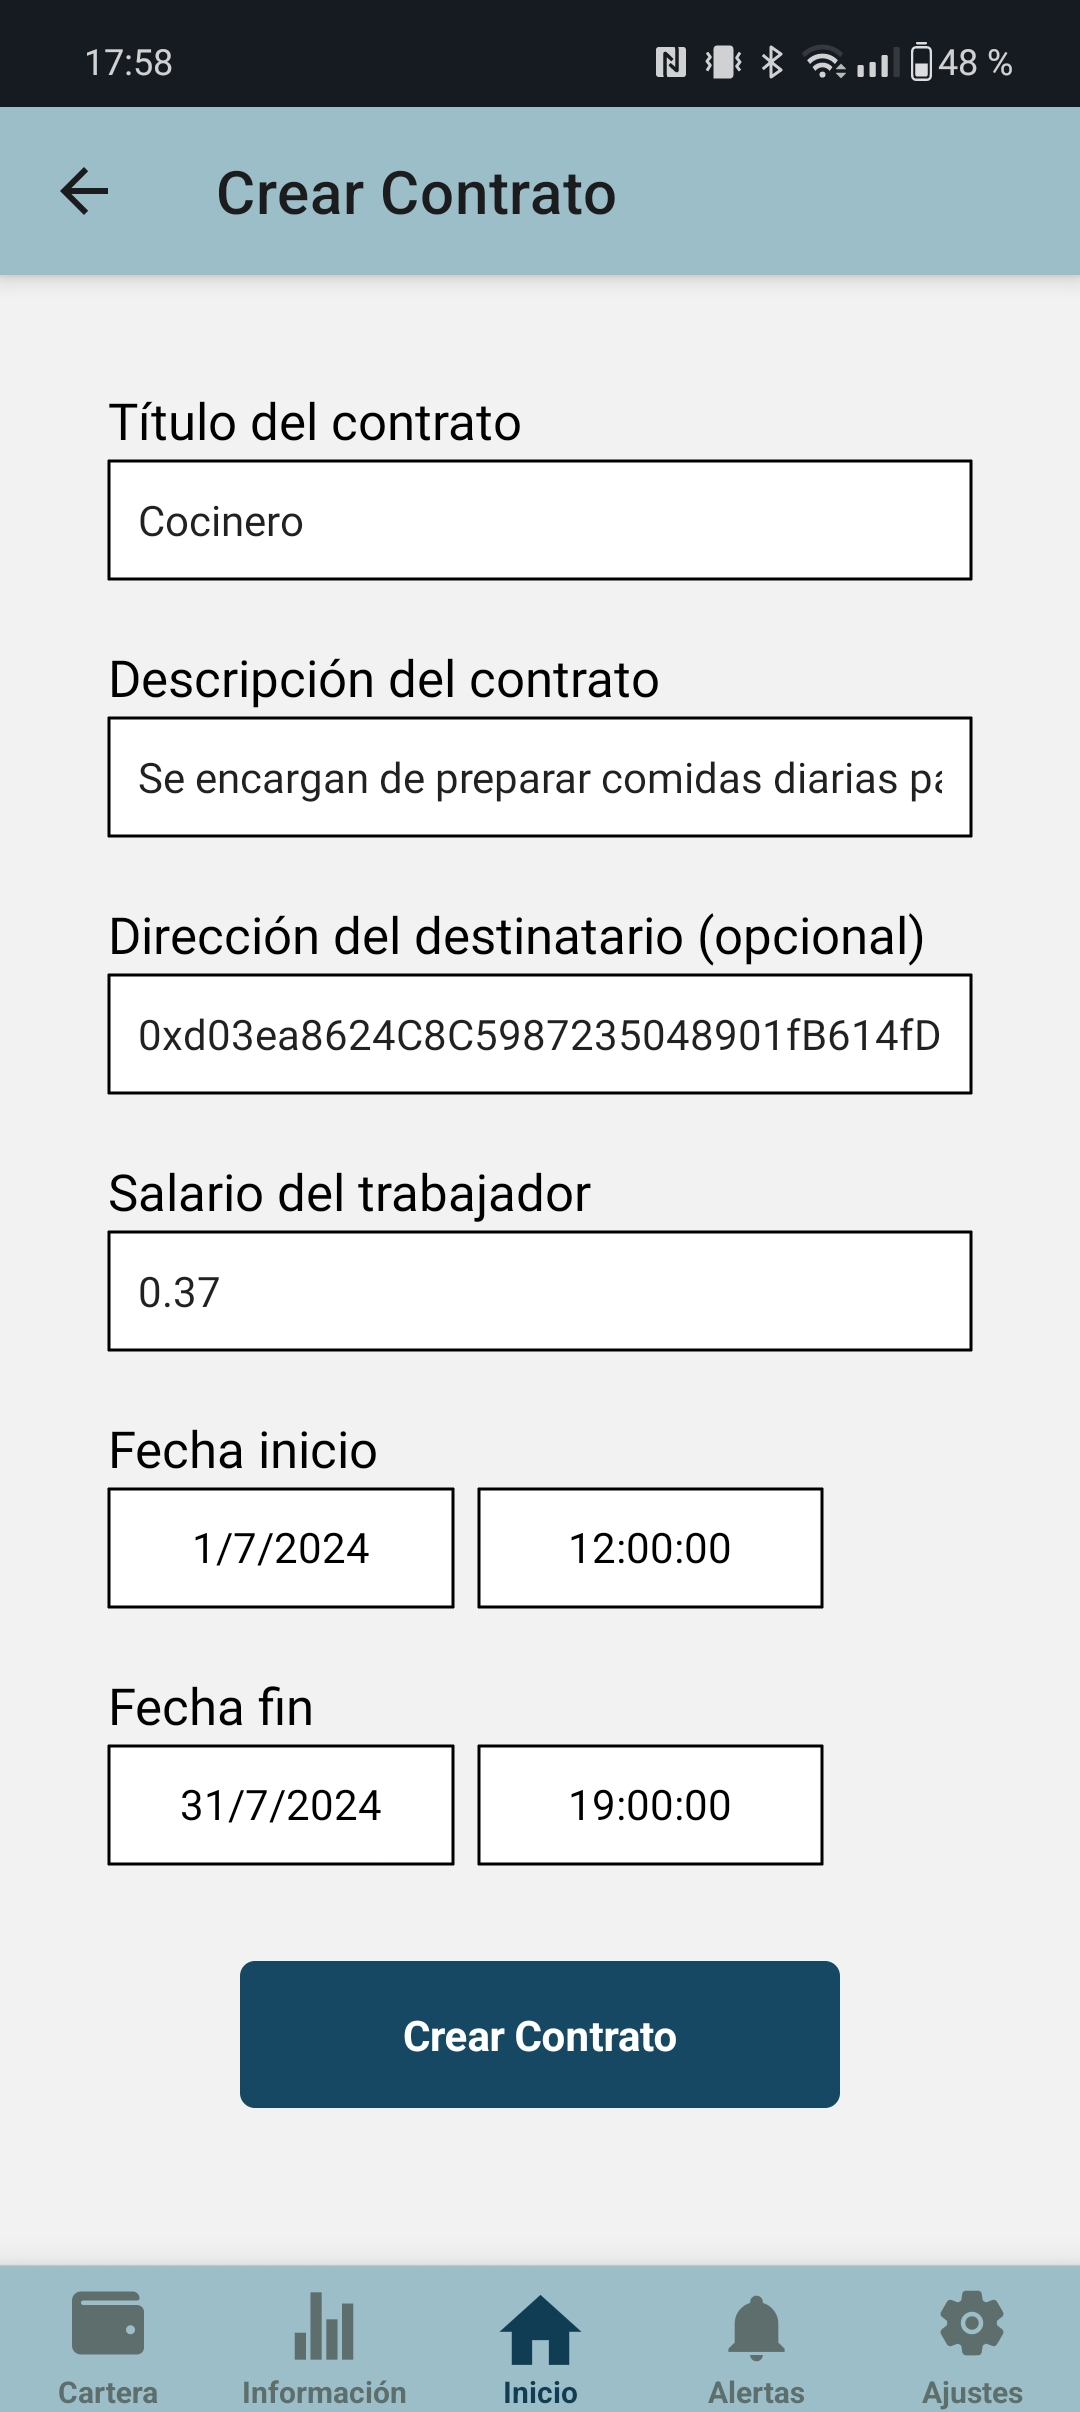
\includegraphics[width=0.40\textwidth]{crearContrato}
	\caption[Pantalla crear contrato]{Pantalla crear contrato.}
\end{figure}


\subsection{Firmar contrato}

La pantalla `Firmar contrato' (imagen \ref{img:firmarContrato}) está diseñada para gestionar la firma de contratos pendientes.
En esta pantalla aparece una lista con los contratos que involucren a un trabajador y todavía no hayan sido firmados.
Al tocar sobre el contrato listado, se redirige al usuario a una nueva pantalla donde se presentan los detalles completos del contrato y finalmente un botón que permite firmar un contrato usando la huella digital o reconocimiento facial.
Por otro lado, también se posibilita al usuario a firmar un contrato mediante un código QR asociado a un contrato específico. Para ello en la parte superior derecha existe un enlace que abre la cámara del dispositivo.
Este método agiliza el proceso de firma asegurando la identificación del usuario.

\begin{figure}[h]
	\label{img:firmarContrato}
	\centering
	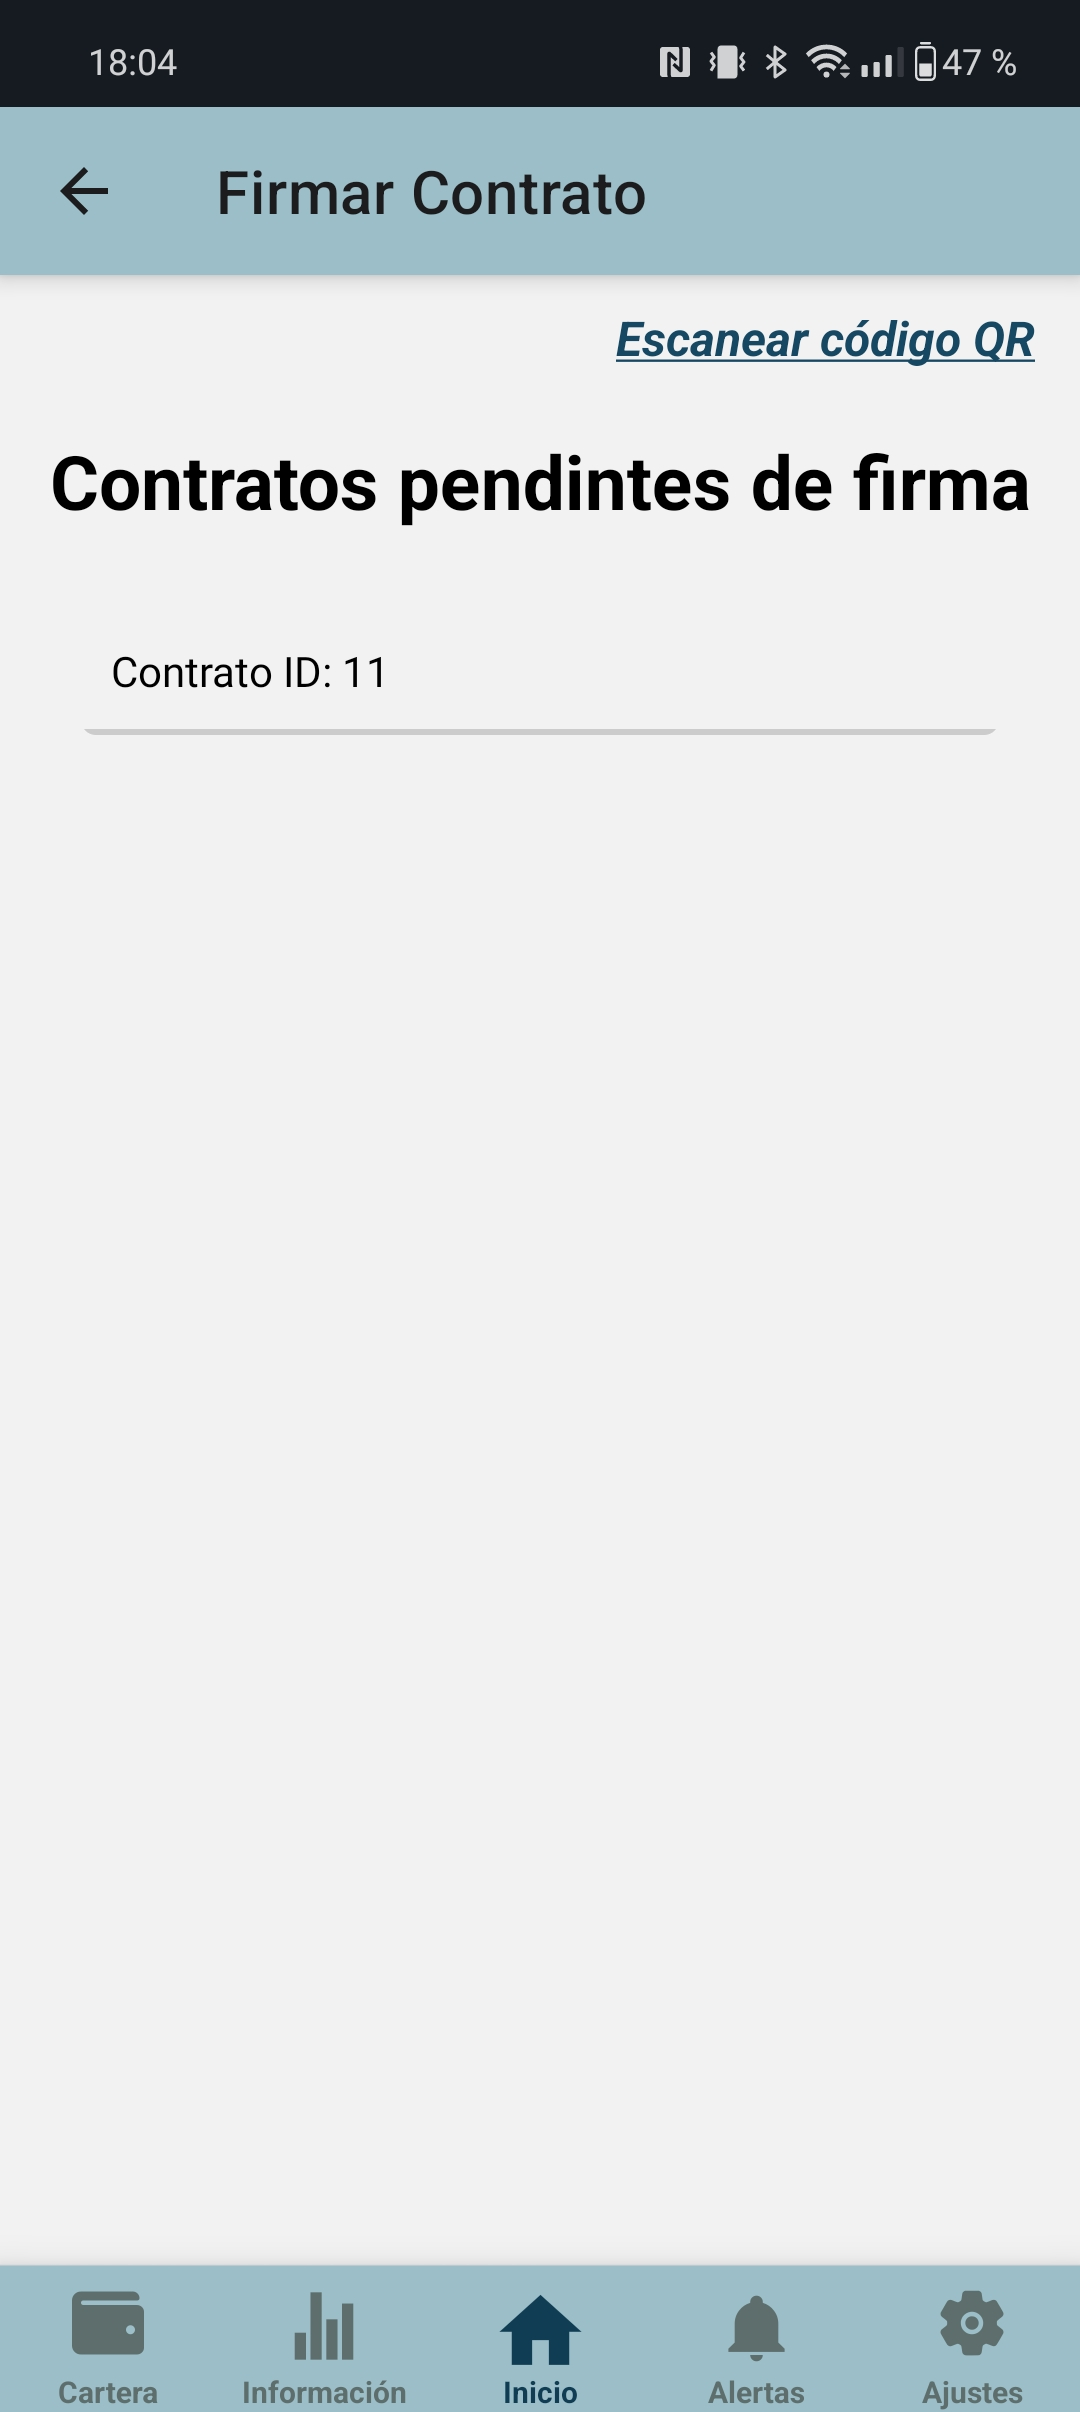
\includegraphics[width=0.40\textwidth]{firmarContrato}
	\caption[Pantalla firmar contrato]{Pantalla firmar contrato.}
\end{figure}


\subsection{Buscar contratos}

Esta pantalla actúa como un tablón de ofertas de trabajo, donde los contratos que aún no tienen asignado un trabajador están listados para que los usuarios puedan explorar y seleccionar oportunidades de empleo según sus intereses y habilidades. 
Este diseño permite a los usuarios tener una visión rápida de las condiciones laborales y la duración de cada contrato. Ver imagen \ref{img:buscarContratos}

En el caso de estar interesado, al seleccionar un contrato específico de la lista, el usuario será dirigido a otra pantalla donde puede ver detalles más extensos del contrato. Desde esta pantalla de información, el usuario tiene la opción de firmar el contrato, facilitando así la conexión entre empleadores y potenciales trabajadores.

\begin{figure}[h]
	\label{img:buscarContratos}
	\centering
	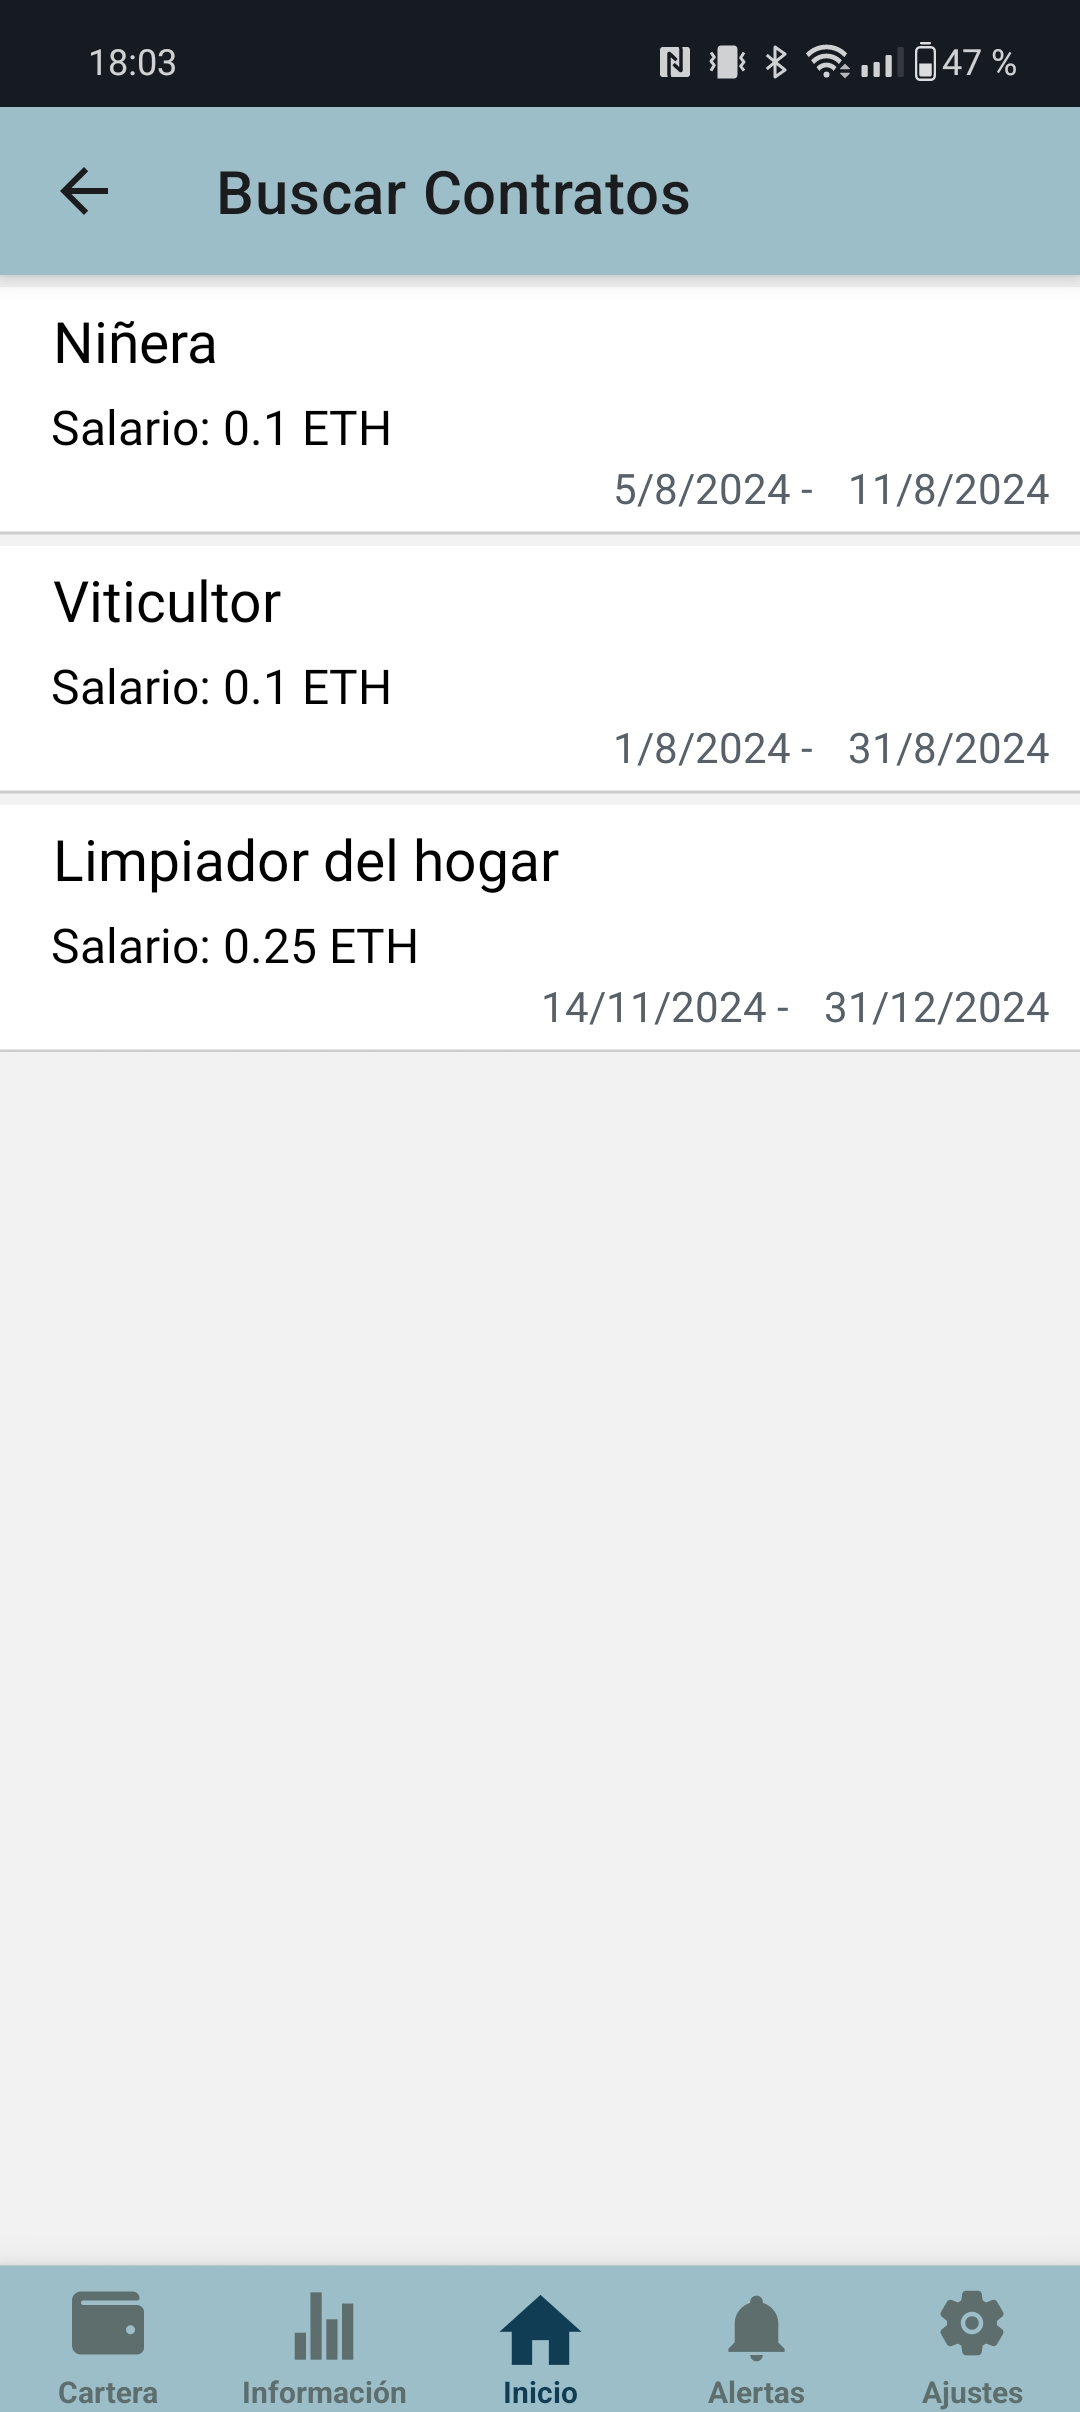
\includegraphics[width=0.40\textwidth]{buscarContratos}
	\caption[Pantalla buscar contratos]{Pantalla buscar contratos.}
\end{figure}



\subsection{Mis contratos}

Esta pantalla (ver imagen \ref{img:misContratos}) esta diseñada para permitir a los usuarios gestionar y revisar los contratos en los que están involucrados, ya se como empleador o como trabajador.
La pantalla incluye dos secciones principales, las cuales han sido etiquetadas como `contratos como empleador' y `contratos como trabajador'. Los usuarios pueden pinchar las etiquetas ubicadas en la parte superior para alternar de una sección a otra, o simplemente deslizar el dedo hacía la derecha o la izquierda.

En la primera sección se muestran todos los contratos iniciados en los que el usuario figura como empleador. En la parte superior aparecerán los contratos que se encuentren activos, mientras que pulsando el botón inferior `Mostrar Contratos Finalizados' se abrirá un desplegable el cual nos permitirá consultar todos los contratos que han expirado.

Por otro lado, en la segunda sección, se muestran los contratos iniciados en los que el usuario figura como trabajador. Del mismo modo que en el caso anterior, en la parte superior aparecerán los contratos que todavía no han finalizado, mientras que en el desplegable inferior se podrá consultar los contratos finalizados.

Al seleccionar cualquier contrato de la lista, el usuario pude acceder a los detalles del mismo y dependiendo del rol que tenga el usuario, tendrá la opción de finalizar el contrato, liberar el salario, realizar una modificación o simplemente consular el contrato.

Esta pantalla está diseñada para ser sencilla y funcional, pudiendo mostrar una gran cantidad de información lo más ordenada y visual posible.

\begin{figure}[h]
	\label{img:misContratos}
	\centering
	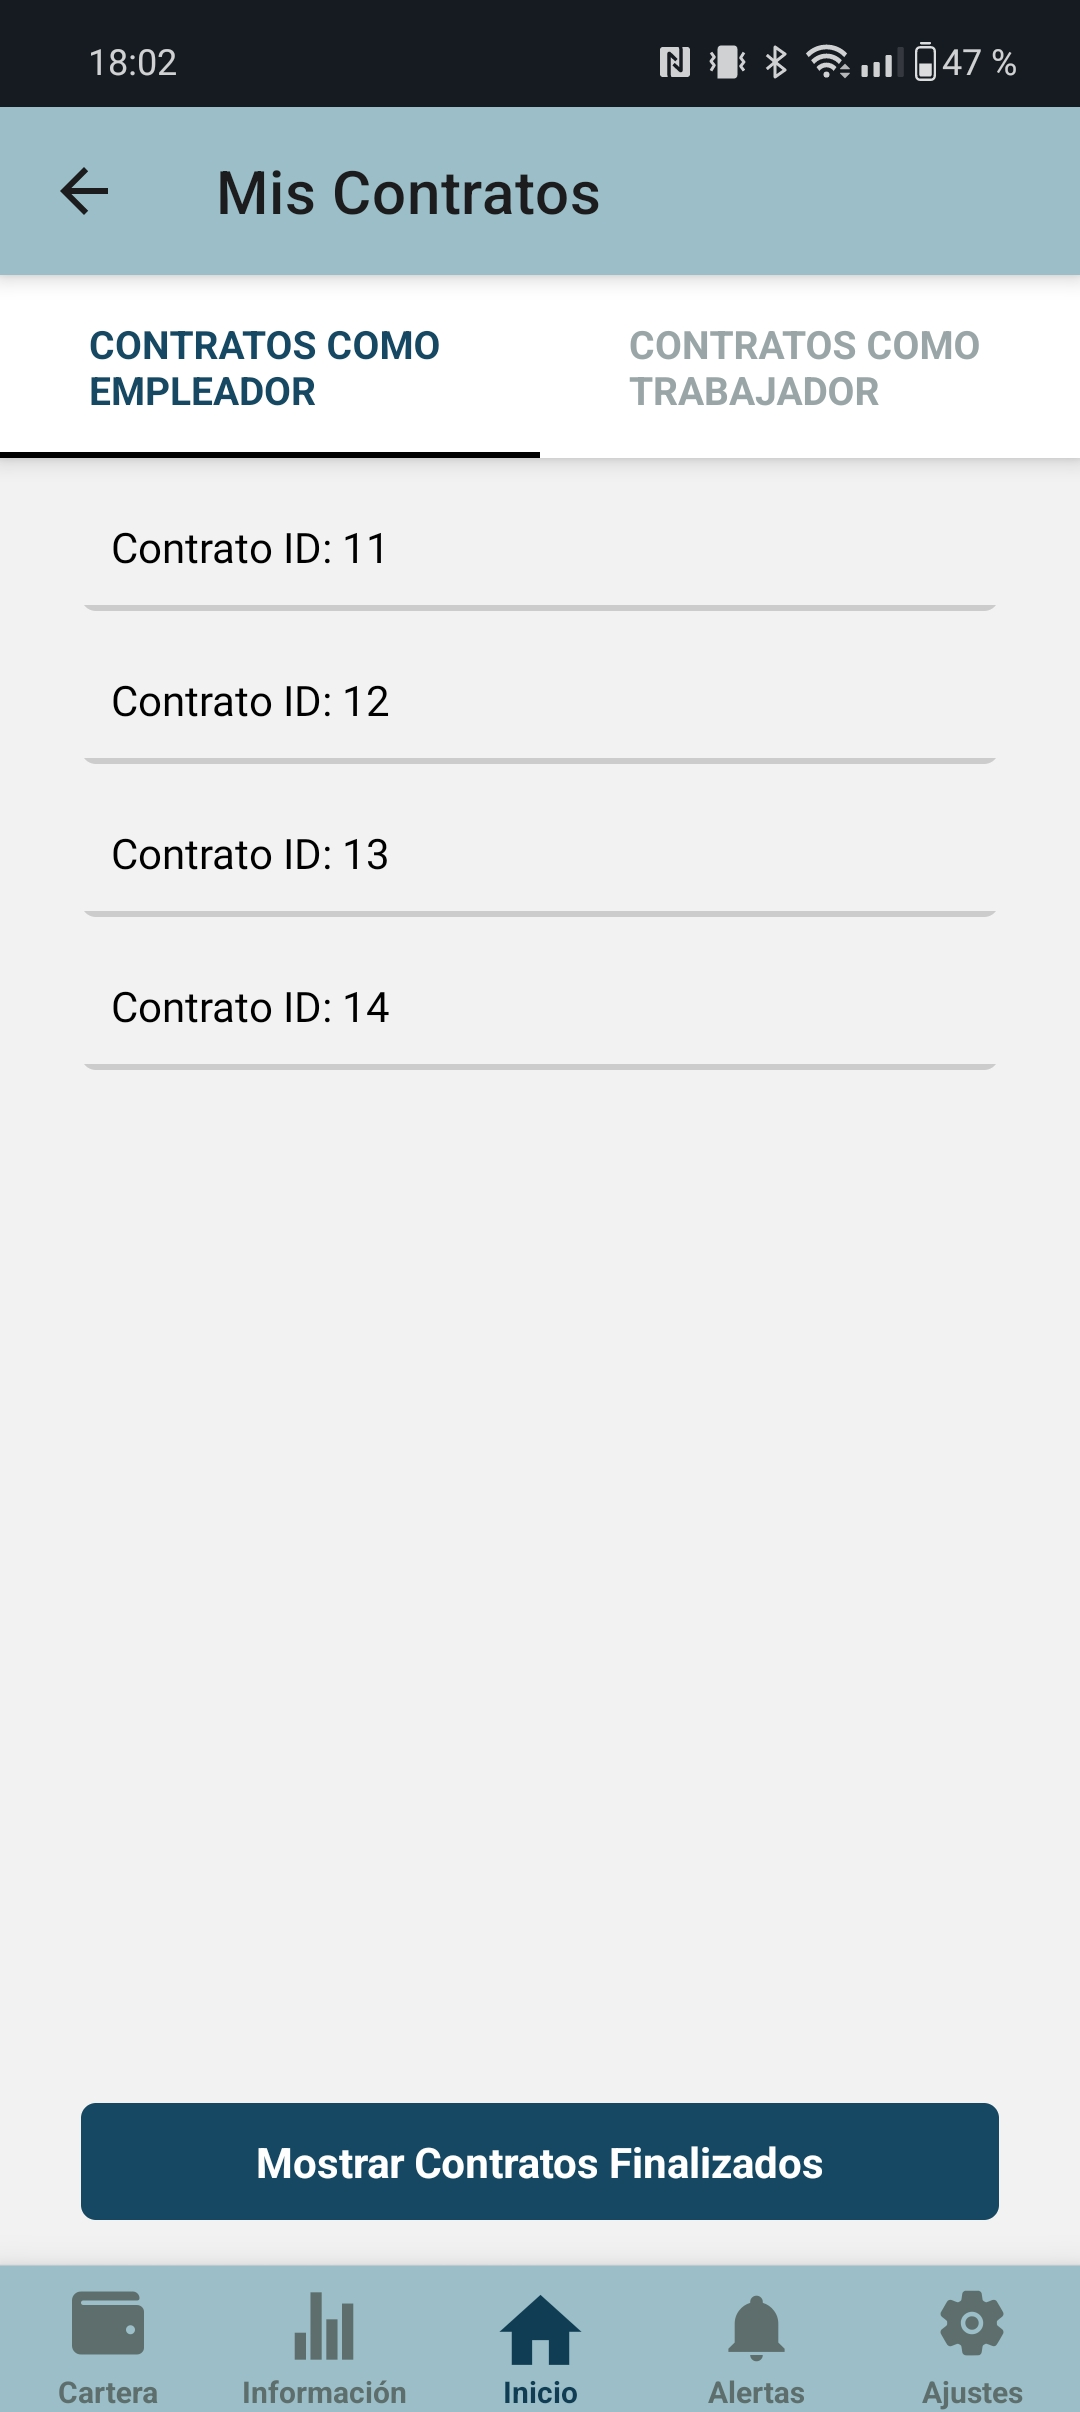
\includegraphics[width=0.40\textwidth]{misContratos}
	\caption[Pantalla contratos del usuario]{Pantalla que muestra los contratos del usuario.}
\end{figure}


\subsection{Detalles contrato}

La pantalla `Consultar Contratos' esta diseñada para permitir a los usuarios consultar todos los detalles de un contrato específico.

Como se puede ver en la imagen \ref{img:infoContrato}, esta pantalla muestra todos los campos explicados previamente en la sección de creación de un contrato. Sin embargo, incluye dos campos adicionales: uno que muestra la billetera del empleador, identificándolo en el proceso, y otro que muestra el estado del contrato. El estado puede ser `pendiente' si el contrato todavía no se ha firmado, `activo' si el contrato se encuentra dentro de las fechas acordadas, `finalizado' si ha superado la fecha de expiración, o `pausado' si se ha decidido pausar el contrato tras una modificación.

Es importante destacar que la imagen presentada en este apartado se ha tomado desde una \textit{tablet} en lugar de un teléfono móvil. Esto se hace con el propósito de demostrar cómo la aplicación se adapta a dispositivos de diferentes tamaños. En el caso de la \textit{tablet}, toda la información se muestra en una sola pantalla sin necesidad de desplazarse. En cambio, en un dispositivo móvil, sería necesario deslizar hacia arriba o hacia abajo para visualizar toda la información.

\begin{figure}[h]
	\label{img:infoContrato}
	\centering
	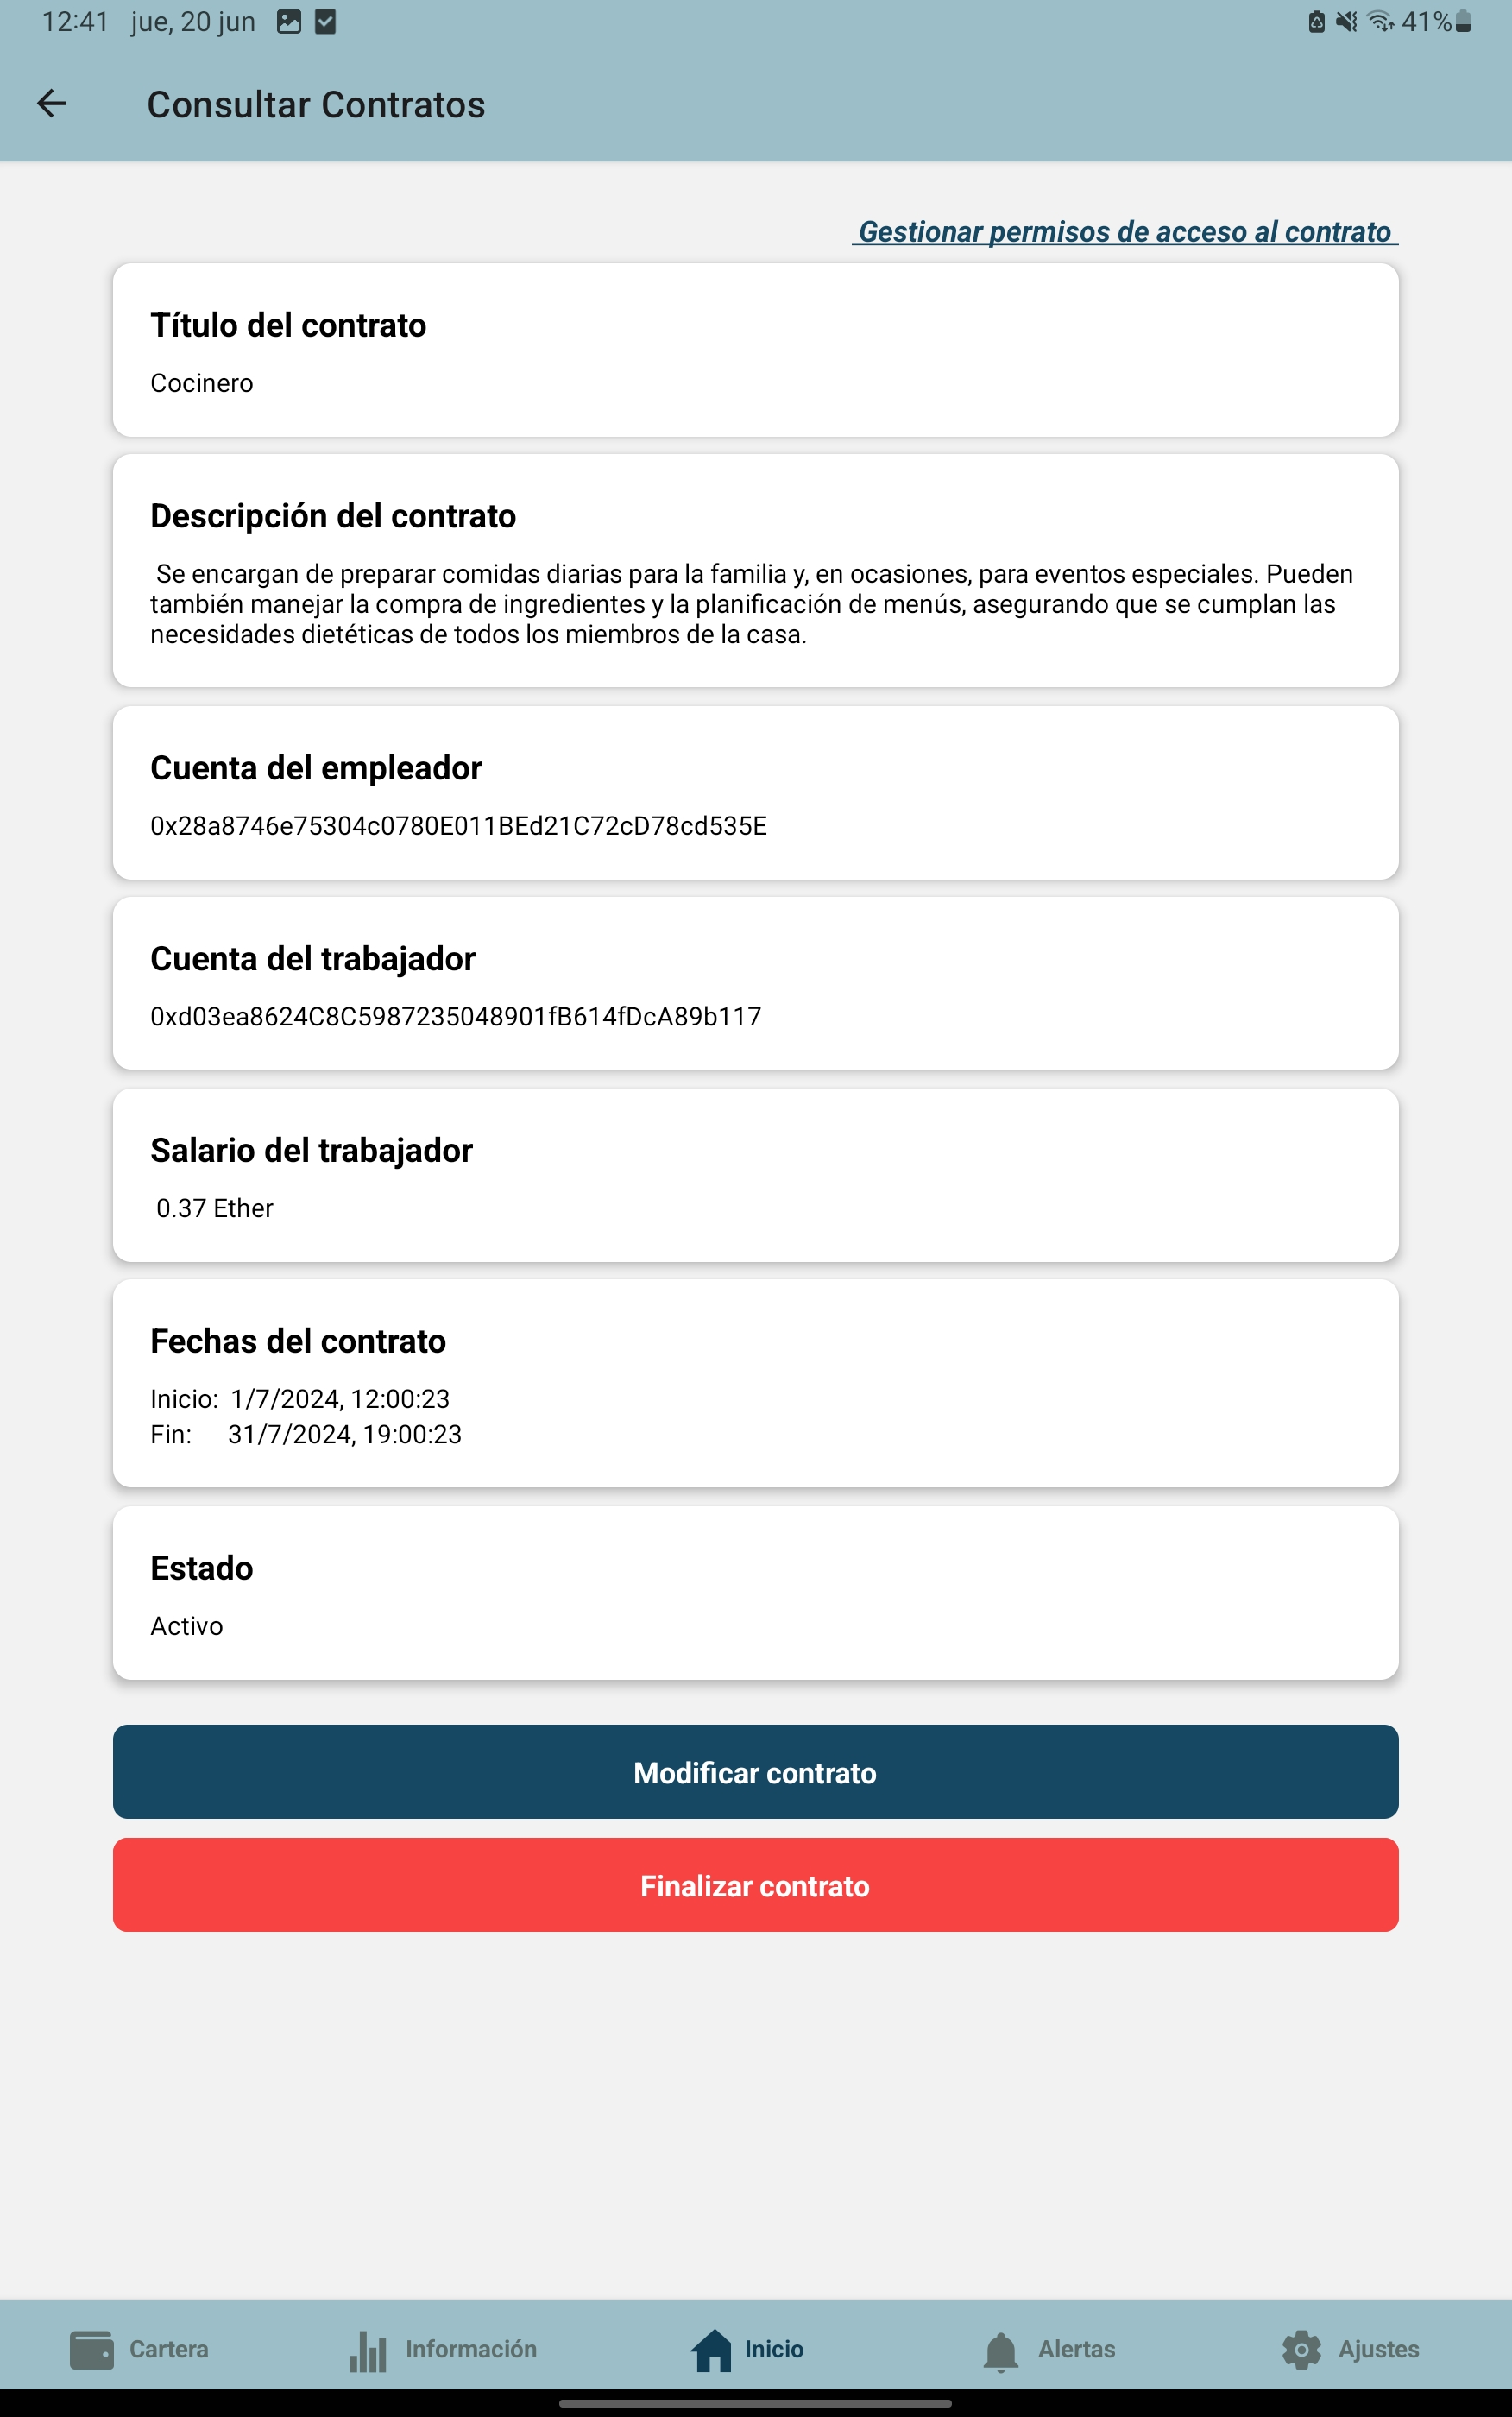
\includegraphics[width=0.50\textwidth]{infoContrato}
	\caption[Pantalla detalles del contrato]{Pantalla que muestra los detalles del contrato.}
\end{figure}

Esta pantalla recoge una gran variedad de funcionalidades, que se mostrarán al usuario dependiendo de su rol en el contrato y del estado actual del mismo.
Para los usuarios que desempeñan el papel de empleadores dentro del contrato, se ofrecen las siguientes opciones:

\begin{itemize}
\item \textbf{Gestión de permisos}: Permite al empleador gestionar y controlar quién puede ver y modificar detalles del contrato.

\item \textbf{Cancelar contrato}: Esta opción solo se encuentra disponible cuando el contrato no ha sido firmado, dando la posibilidad al usuario de cancelar el contrato y recuperar el dinero depositado en el mismo.

\item \textbf{Modificar contrato}: Facilita la actualización de los términos del contrato cuando este se encuentre activo. Se enviará una propuesto con los cambios sugeridos que tendrá que ser aprobada por el trabajador.

\item \textbf{Finalizar contrato}: Permite al empleador cerrar formalmente el contrato antes de su fecha de expiración si se considera que todas las obligaciones han sido cumplidas, marcando el final del compromiso laboral.

\item \textbf{Liberar pago}: Cuando el contrato se encuentre finalizado, se habilita esta opción para que el empleador pueda liberar el pago del salario al trabajador.
\end{itemize}

Por otro lado, desde la perspectiva del trabajador, además de poder consultar los detalles completos del contrato, dispondrá de la funcionalidad exclusiva de revisar cualquier propuesta de modificación del contrato. Esta opción se activa solo cuando existen cambios pendientes de revisión, permitiendo al usuario acceder a una pantalla donde evaluar los cambios y responder a la modificación sugerida.


\subsection{Modificar Contrato y aprobar cambios}

En este apartado se presentan dos funciones interrelacionadas. La primera es la modificación de un contrato, como se ilustra en la primera pantalla de la imagen \ref{img:modificarCambios}. 
Una vez el contrato se encuentre firmado, el empleador tiene la posibilidad de proponer modificación a los términos del contrato existente. 

Los aspectos a modificar recogen:
\begin{itemize}

\item \textbf{Título}: Actualización del título del contrato.

\item \textbf{Descripción}: Ajuste de los detalles del contrato.

\item \textbf{Salario}: modificación de la cantidad del salario: si se incrementa, será necesario depositar la nueva cantidad al contrato, mientras que si se decrementa, la diferencia será devuelta al empleador. 

\item \textbf{Duración}: Permite modificar la fecha de finalización del contrato.

\item \textbf{Pausa del contrato}: Posibilidad de pausar temporalmente el contrato. Al reactivarse, se añadirá al contrato el tiempo que estuvo pausado.

\end{itemize}

Tras enviar la propuesta de modificación, el trabajador recibirá una alerta que le notificará que hay cambios propuestos. Al acceder a la segunda pantalla de la imagen \ref{img:modificarCambios}, se puede observar en verde los detalles modificados respecto a los términos originales. Después de revisar estos cambios, el trabajador tendrá la opción de aceptar o rechazar los cambios propuestos, asegurando así su acuerdo antes de que los cambios se efectúen.

\begin{figure}[h]
	\label{img:modificarCambios}
	\centering
	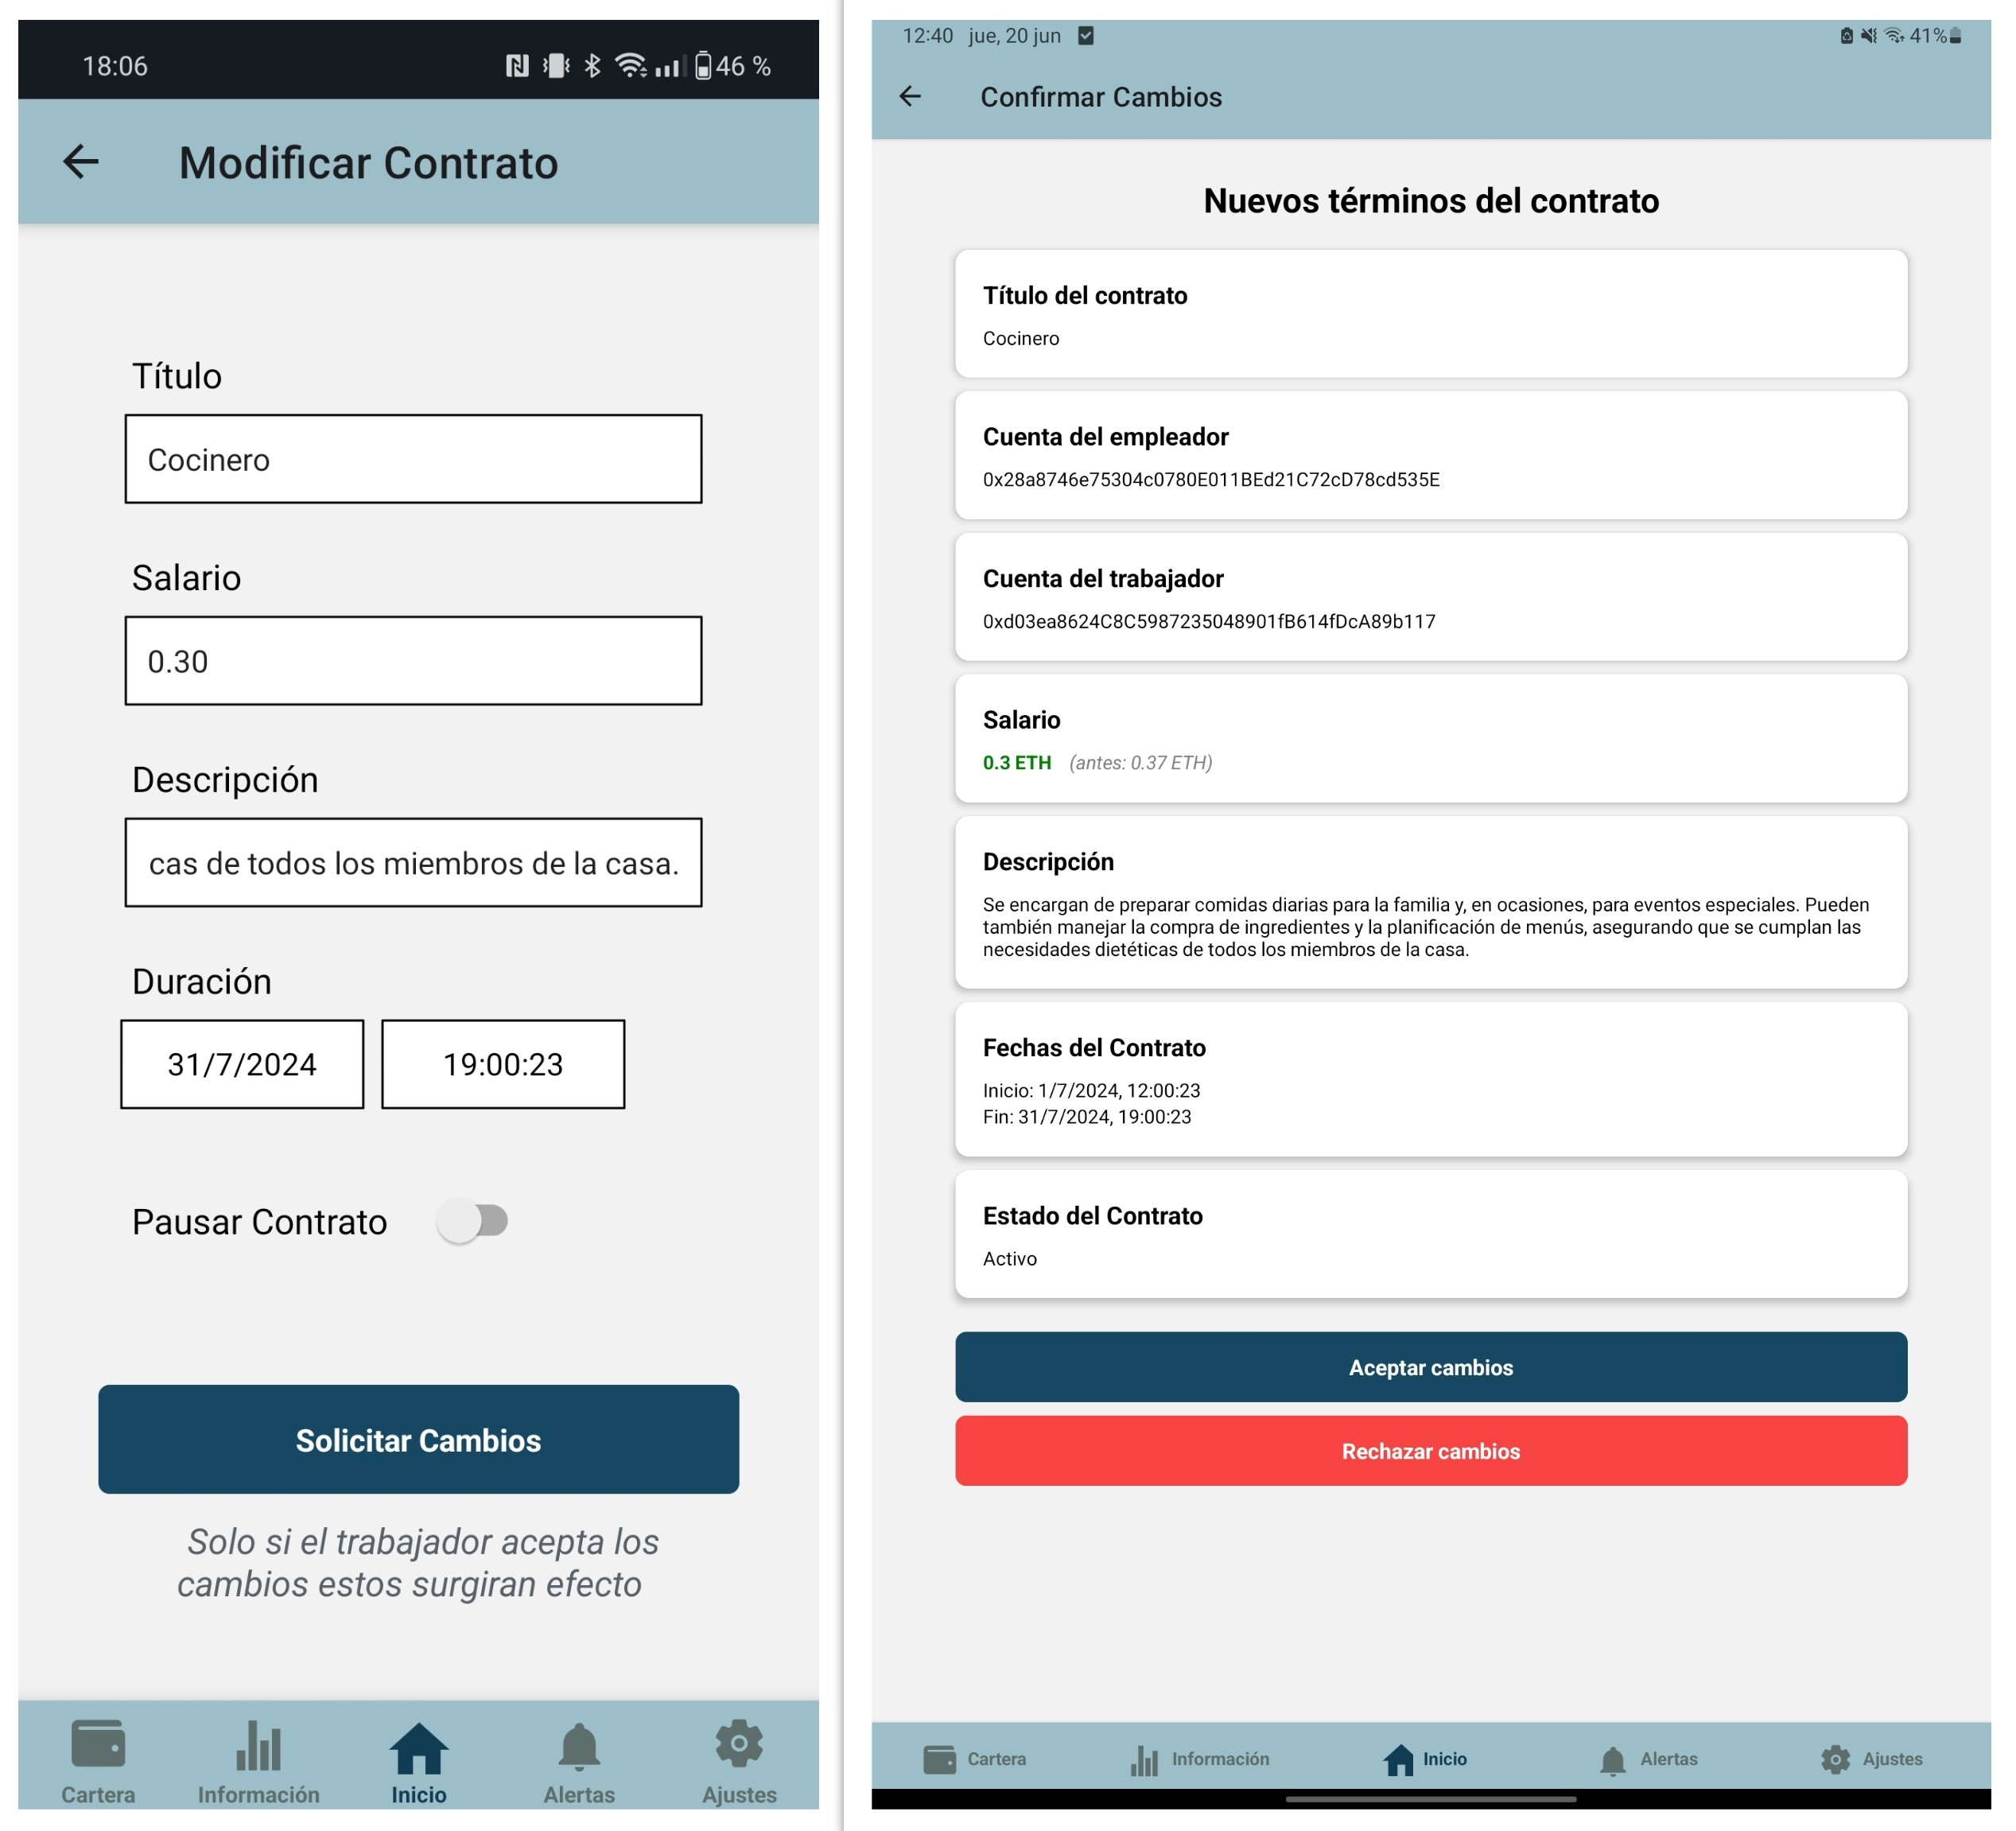
\includegraphics[width=0.90\textwidth]{modificarCambios}
	\caption[Pantalla modificar contrato]{Pantallas de propuesta de modificación y aprobación de cambios.}
\end{figure}


\subsection{Añadir manager y código QR}

Como mencionó en apartados anteriores, dos de las funcionalidades destacadas en la pantalla de detalles del contrato incluyen la adición de un tercero para su gestión y la visualización del código QR para la firma del contrato.

En la primera pantalla, ver imagen \ref{img:managerQR}, está diseñada para otorgar permisos de visualización y gestión sobre un contrato a un usuario designado.
Para ello, el empleador introduce la dirección de la billetera del usuario deseado, y luego lo asigna pulsando el botón `Asignar Manager'.
Una vez asignado, el nuevo \textit{manager} se añade a una lista de \textit{managers} actualmente asignados. Desde esta lista, del mismo modo se pude borrar un \textit{manager} pulsando un emoticono que representa una papelera.

la segunda pantalla de la imagen \ref{img:managerQR}, se visualiza al presionar el botón `Mostrar Código QR' desde la pantalla \ref{img:infoContrato}.
Esta opción está disponible únicamente cuando el contrato aún no ha sido firmado. Al activar esta función, se genera un código QR, como se observa en la pantalla. La descripción bajo el código explica que, al escanear este código QR, el contrato será automáticamente firmado por el usuario que realiza el escaneo.

\begin{figure}[h]
	\label{img:managerQR}
	\centering
	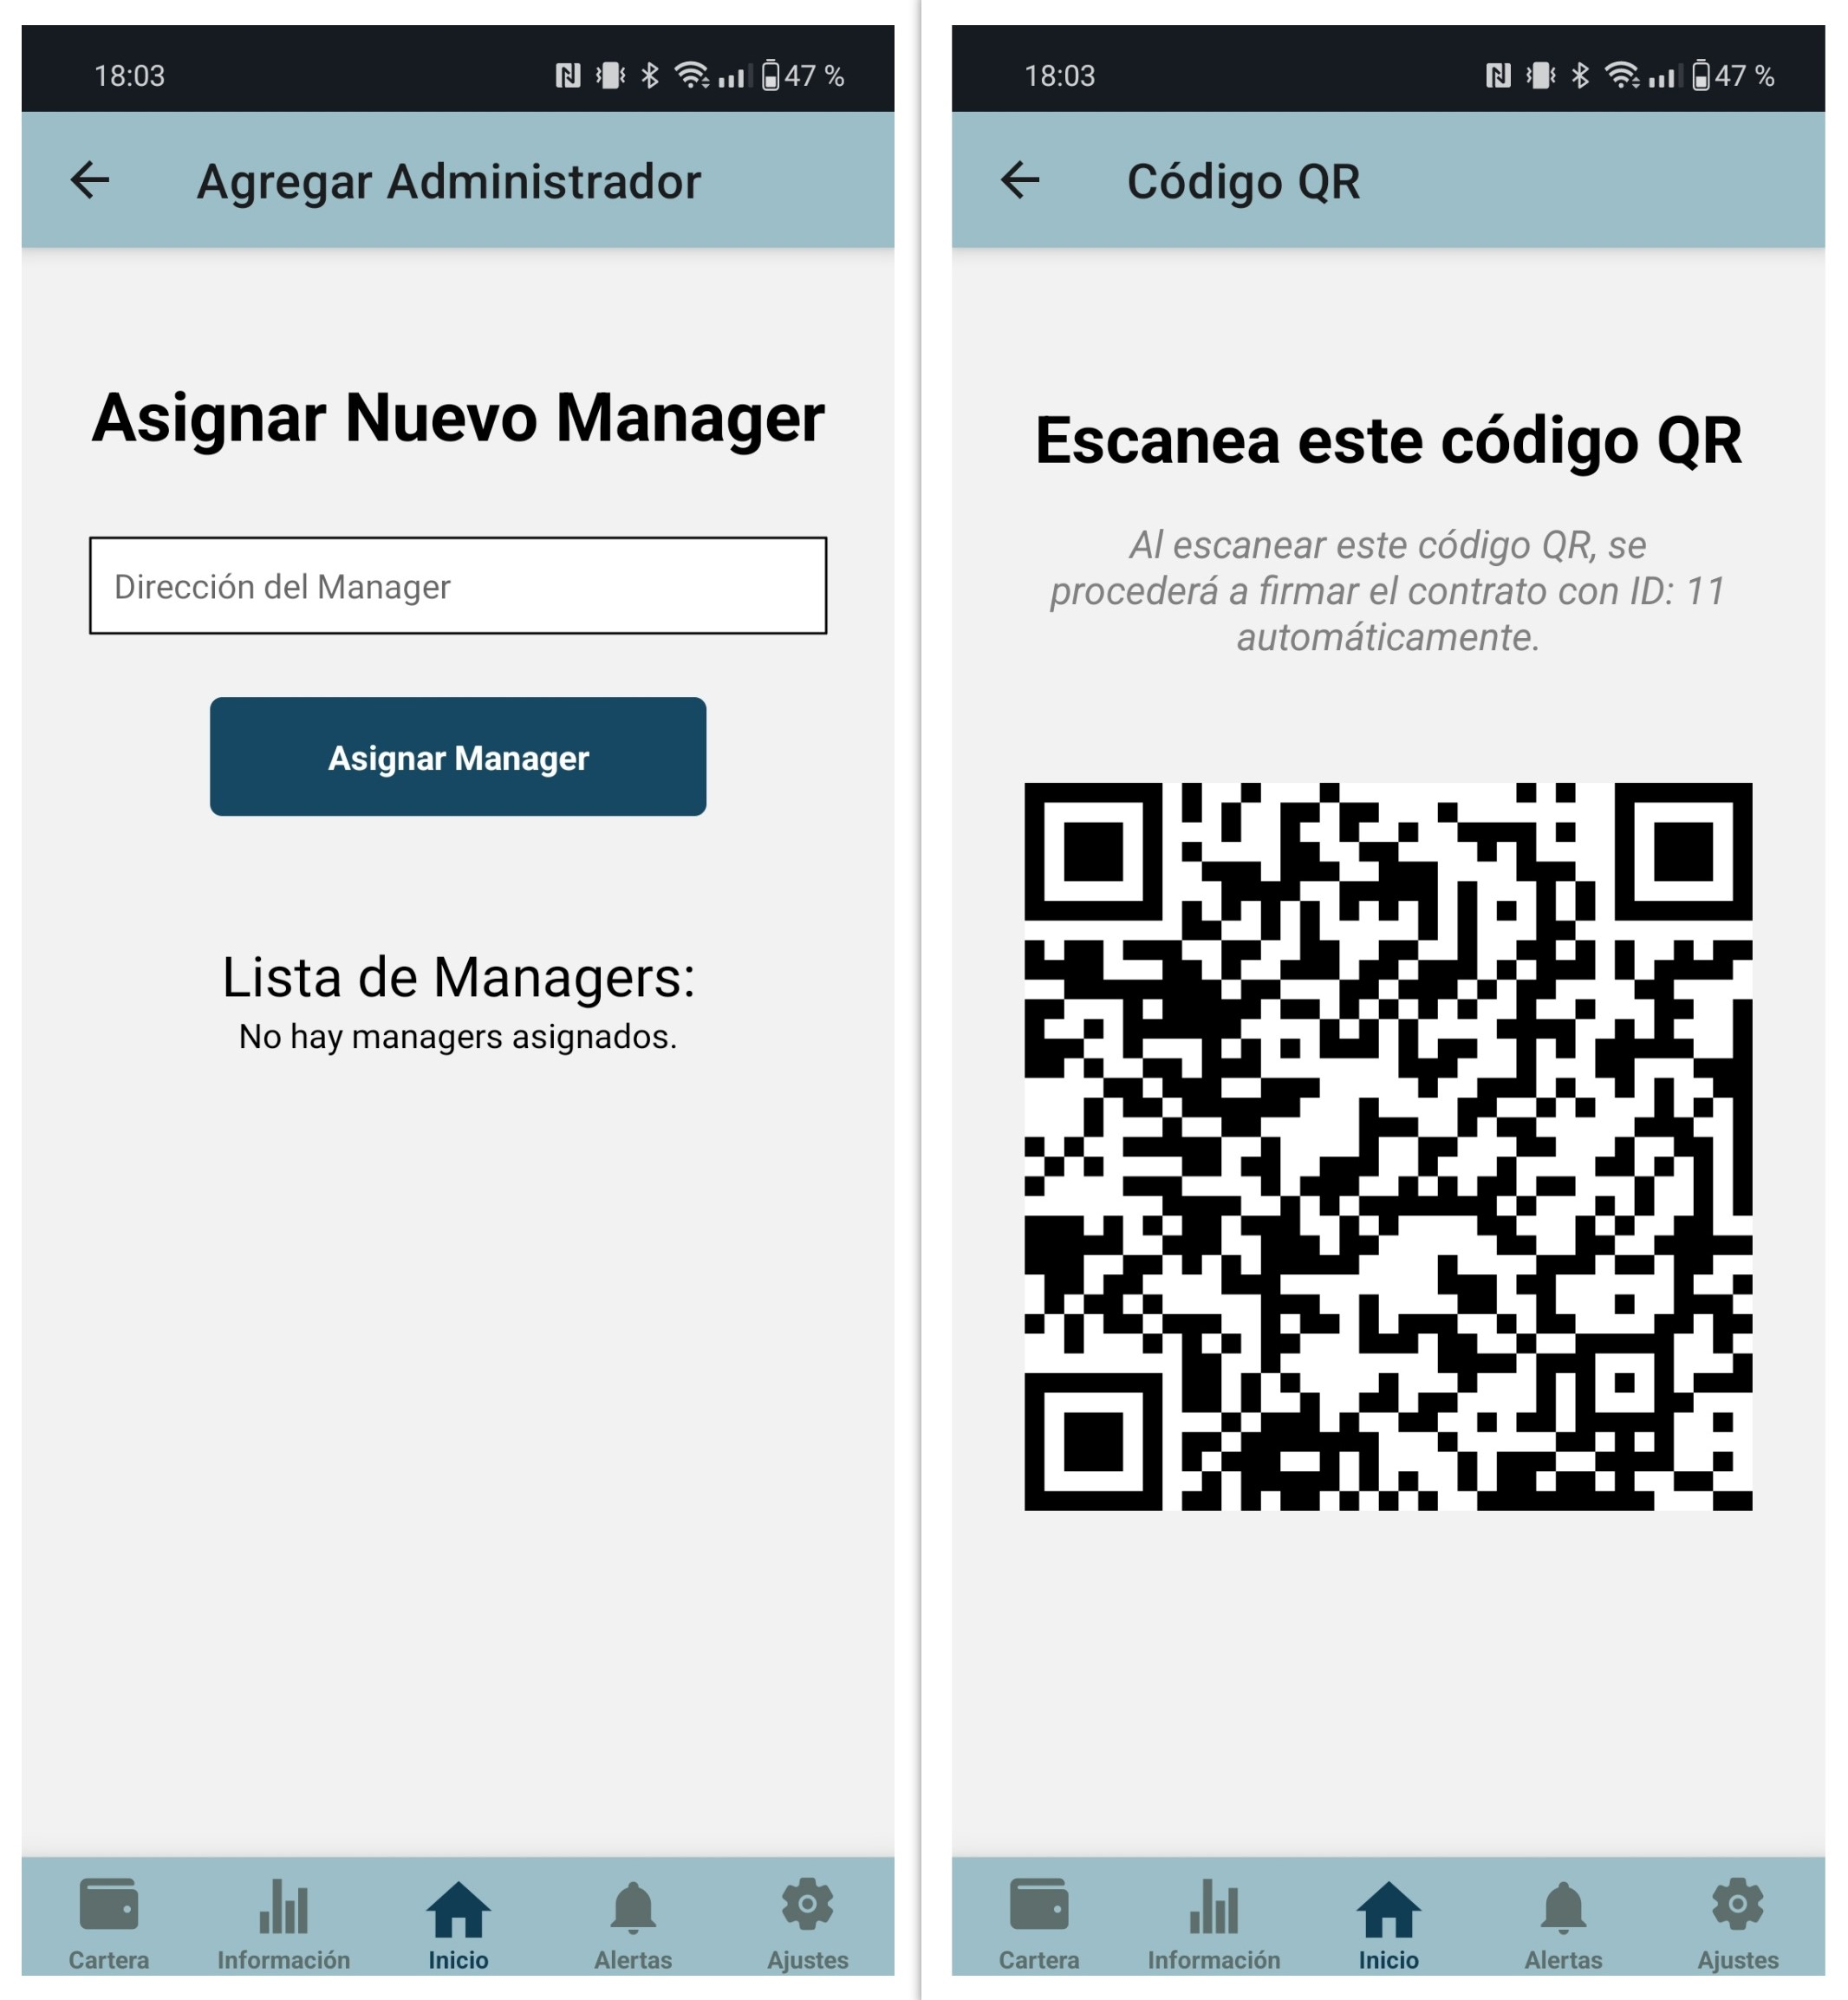
\includegraphics[width=0.90\textwidth]{managerQR}
	\caption[Pantalla añadir manager y código QR]{Pantallas de gestión de acceso y código QR de un contrato.}
\end{figure}


\subsection{Alertas}

La pantalla \ref{img:alertas}, sirve como centro de notificaciones para el usuario, mostrando todos los eventos relacionados con sus contratos.
Cada alerta muestra el ID del contrato al que pertenece, lo que permite una rápida identificación y seguimiento. Además, al seleccionar cualquiera de las alertas, el usuario puede acceder directamente al contrato en cuestión para ver detalles adicionales.

Las alertas que puede recibir un usuario son las siguientes:
\begin{itemize}
\item \textbf{Creación de contrato}: Notifica al usuario cuando es agregado como trabajador a un nuevo contrato.

\item \textbf{Firma de contrato}: informa al empleador cuando el contrato ha sido firmado.

\item \textbf{Liberación de salario}: Avisa cuando el empleador ha liberado el salario correspondiente al contrato.

\item \textbf{Cancelación de contrato}: Alerta cuando un contrato ha sido cancelado por el empleador.

\item \textbf{Finalización de contrato}: Notifica cuando un contrato ha sido concluido por el empleador.

\item \textbf{Propuesta de modificación}: Se informa al usuario cuando el empleador sugiere una modificación al contrato.

\item \textbf{Aceptación o rechazo de modificación}: informa al empleador si su propuesta de modificación ha sido aceptada o rechazada.
\end{itemize}

\begin{figure}[h]
	\label{img:alertas}
	\centering
	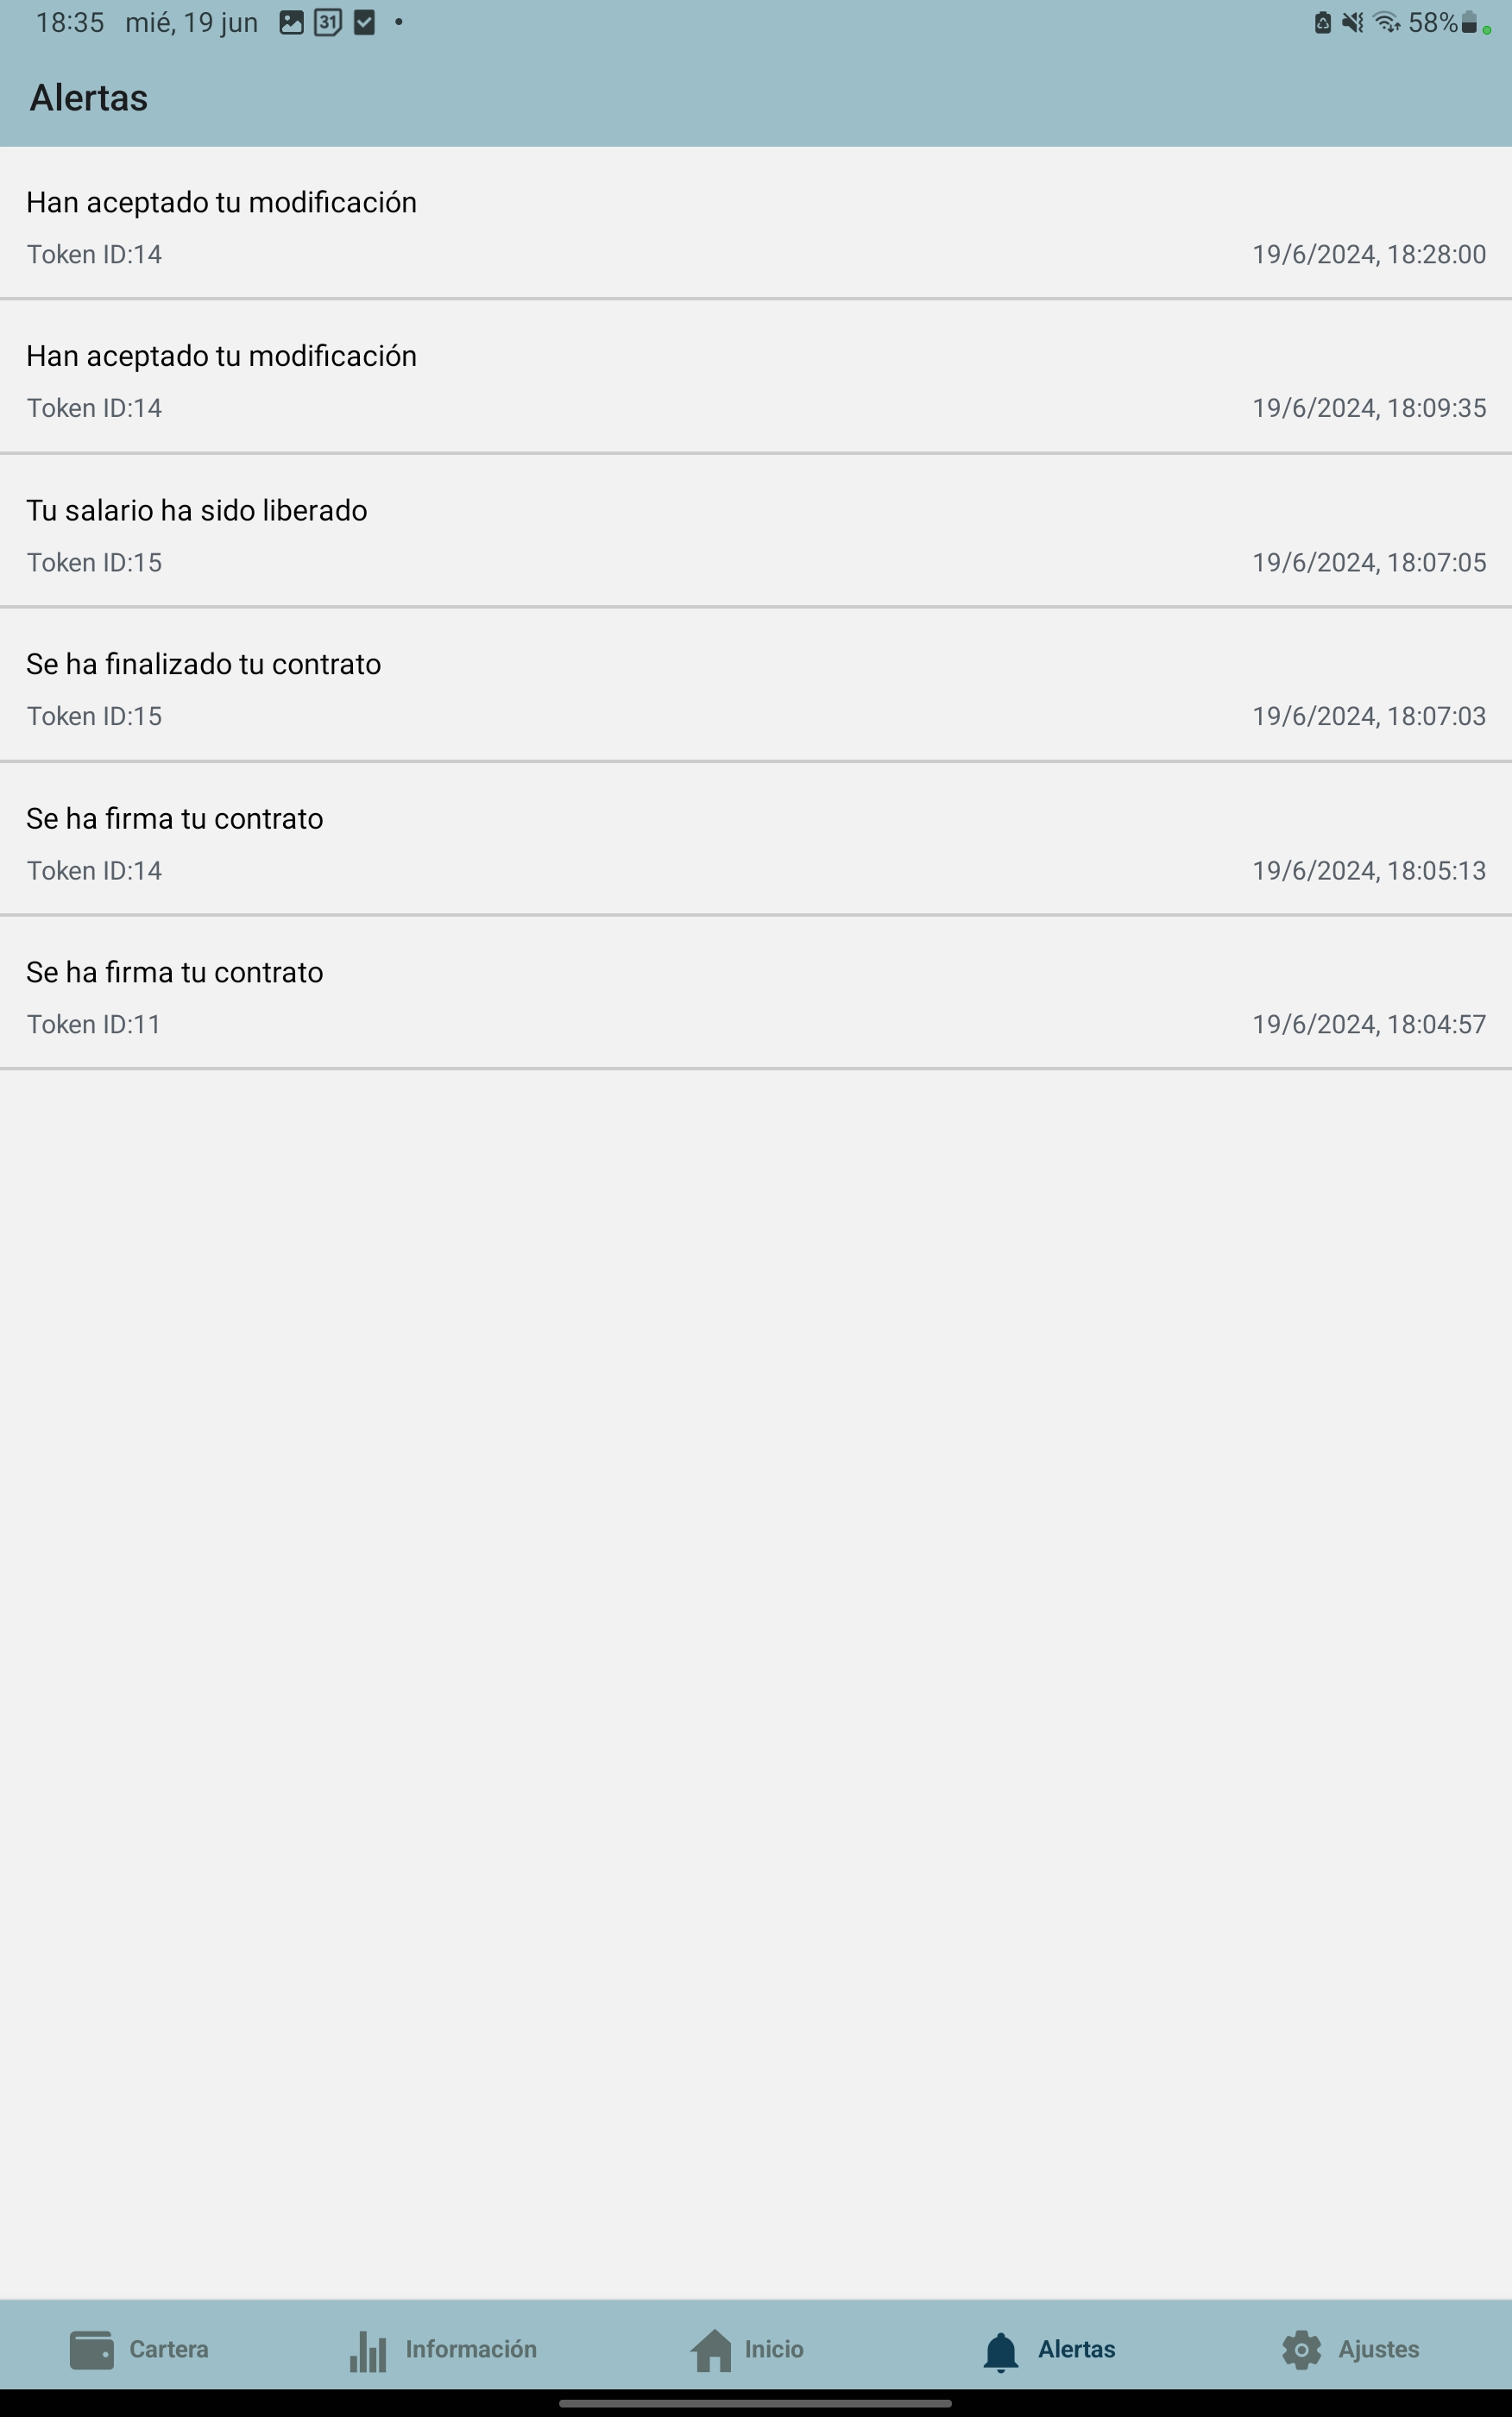
\includegraphics[width=0.50\textwidth]{alertas}
	\caption[Pantalla alertas]{Pantalla de notificación de alertas.}
\end{figure}



\subsection{Cartera}

La siguiente pantalla (ver imagen \ref{img:cartera}) ofrece un seguimiento detallado de las transacciones financieras dentro de la aplicación.
Lo primero que se muestra en esta pantalla es la dirección de la billetera del usuario actual, seguido del saldo actual en Ether (ETH) de la cuenta.
Seguidamente, se registra cada transacción financiera en la que el usuario ha estado involucrado, detallando a qué contrato pertenece cada una, así como la fecha y hora exactas en que se realizó.

Por un lado, las transacciones que representar un gasto se deben principalmente a dos escenarios: primero, cada vez que se crea un nuevo contrato, se efectúa un depósito inicial; segundo, si se incrementa el salario de un trabajador durante una modificación contractual, esto también resulta en una deducción adicional para cubrir dicho aumento.

Por otro lado, los ingresos pueden surgir de varias maneras: los usuarios reciben dinero cuando se libera el salario, ya sea por la finalización por parte del empleador o porque haya expirado. Además, si un contrato se cancela o el salario se reduce, esto también resulta en la devolución de los fondos sobrantes.

\begin{figure}[h]
	\label{img:cartera}
	\centering
	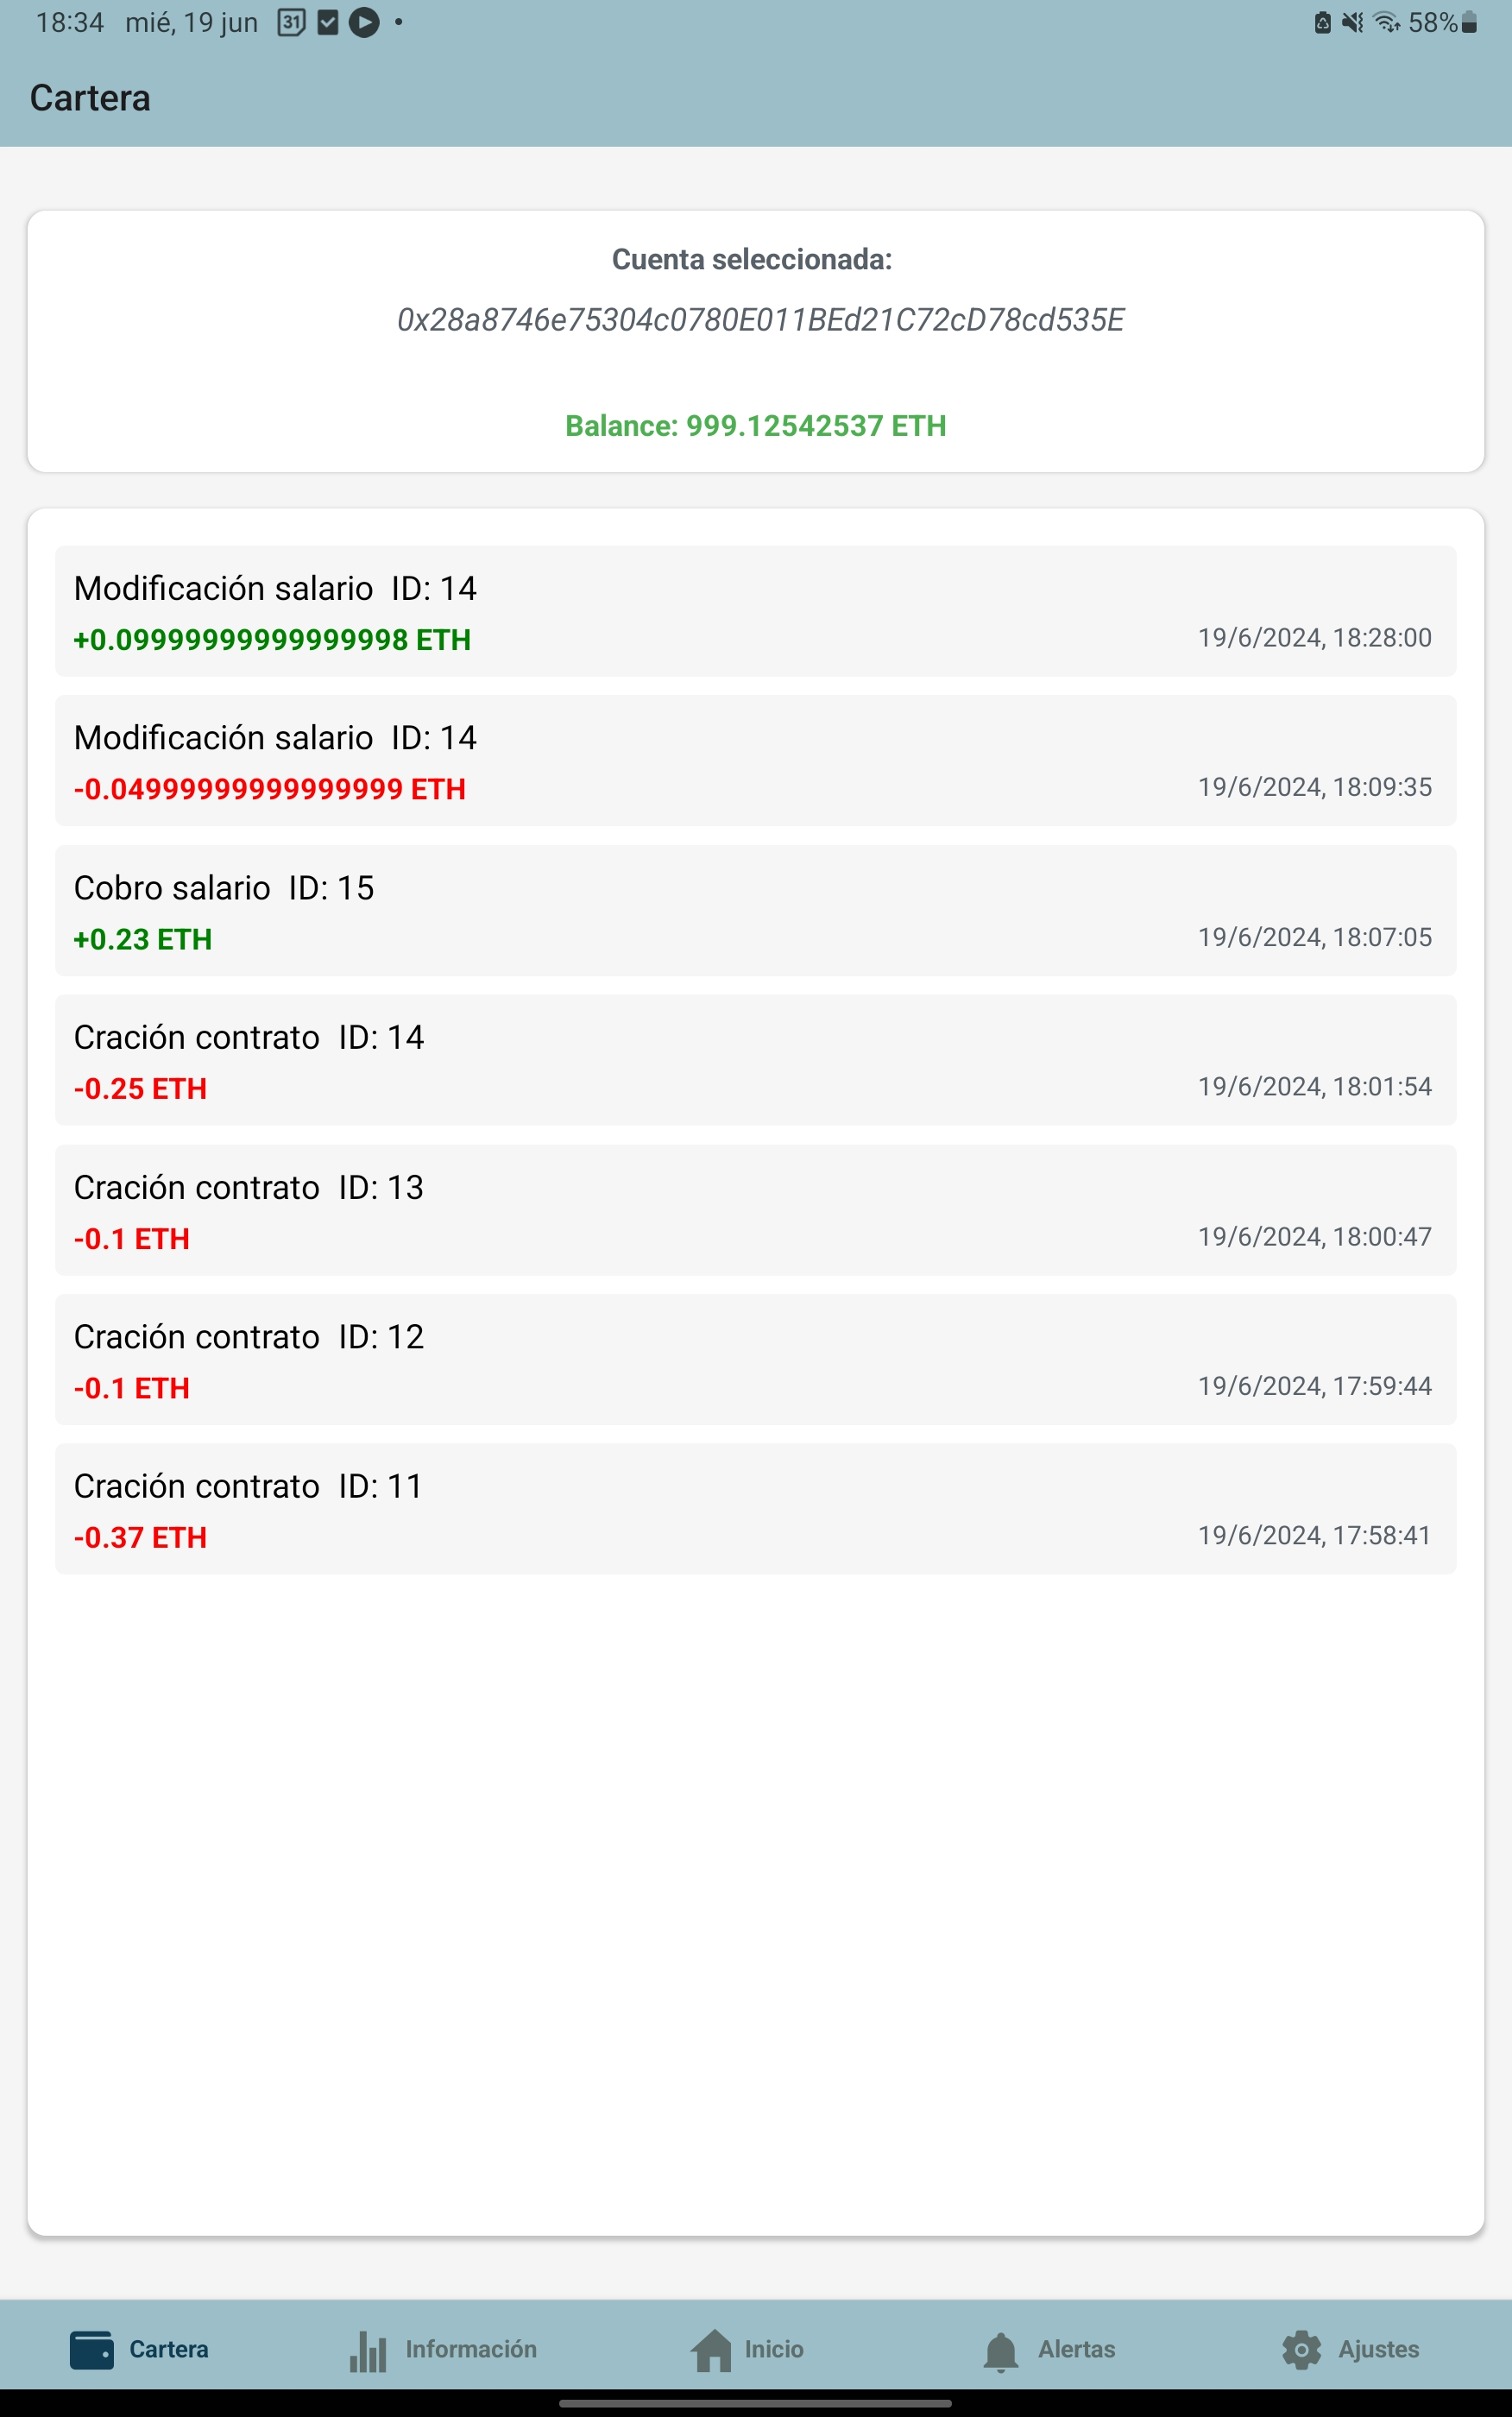
\includegraphics[width=0.50\textwidth]{cartera}
	\caption[Pantalla cartera]{Pantalla que muestra activos y últimos movimientos de la cuenta.}
\end{figure}



\subsection{Pantalla utilidades}

La pantalla \ref{img:infoHerramientas} está diseñada específicamente para facilitar a los usuarios la gestión y operación con Ethereum.
Esta pantalla proporciona una herramienta que incluye tanto información actualizada sobre el precio del Ethereum en euros como un análisis histórico del mismo a través de un gráfico que rastrea el precio a lo largo del último año.

En la parte inferior de la pantalla, se encuentra un conversor de divisas que permite a los usuarios calcular rápidamente el equivalente de una cantidad dada de euros en Ethereum, y viceversa. Para alternar entre la conversión de euros a Ethereum y de Ethereum a euros, los usuarios simplemente deben pulsar el icono de cambio situado junto a los campos de entrada.
La funcionalidad del conversor es intuitiva, al introducir una cifra en el campo, la conversión se realiza automáticamente, utilizando la tasa de cambio más reciente reflejada en el indicador del precio actual. 

\begin{figure}[h]
	\label{img:infoHerramientas}
	\centering
	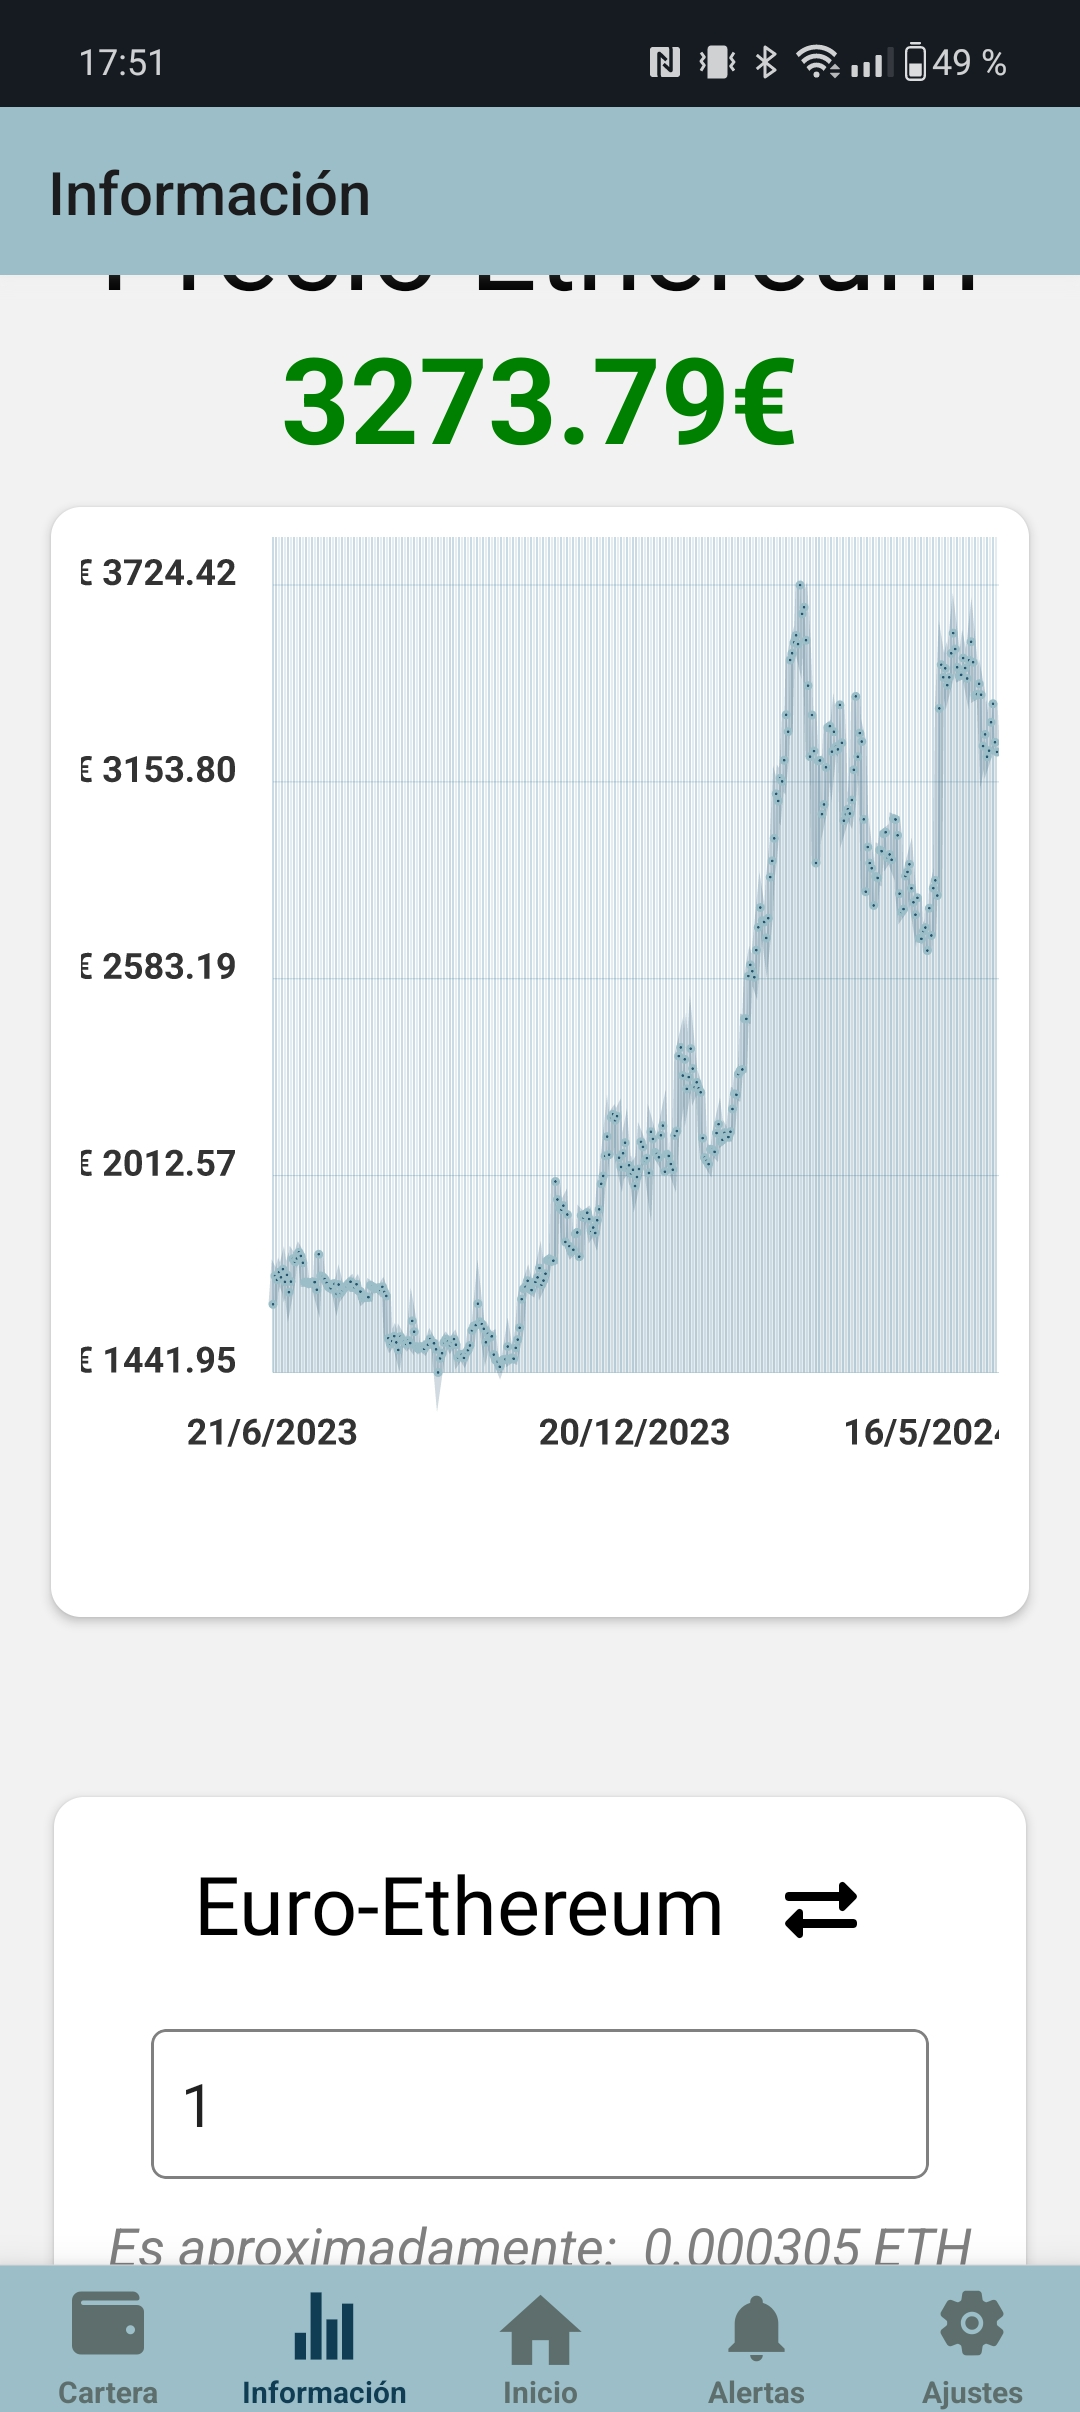
\includegraphics[width=0.40\textwidth]{infoHerramientas}
	\caption[Pantalla utilidades]{Pantallas de información y herramientas.}
\end{figure}


\subsection{Perfil}

La primera pantalla mostrada en la imagen \ref{img:perfilModificar}, ofrece al usuario una vista detallada de su perfil, ofreciendo detalles como:

\begin{itemize}
\item \textbf{Nombre}: El nombre completo del usuario.

\item \textbf{Email}: La dirección de correo electrónico asociada con la cuenta.

\item \textbf{DNI}: Número de identificación del usuario.

\item \textbf{Fecha de Nacimiento}: Presentada en el formato día/mes/año.

\item \textbf{Dirección}: Incluye la dirección completa, señalando la calle y ciudad.

\item \textbf{Teléfono}: Número de contacto del usuario.

\item \textbf{Ganache Address}: Dirección de la billetera del usuario.
\end{itemize}

En la parte inferior de la pantalla se encuentra el botón `cerrar sesión', este botón permite al usuario cerrar su sesión activa, garantizando la seguridad de la cuenta. Si el usuario no cierra sesión, su cuenta permanecerá abierta para un acceso rápido en futuras visitas.

Por otro lado, el botón `Modificar perfil' redirige al usuario la pantalla de modificación del perfil (imagen \ref{img:perfilModificar}).
Esta pantalla ofrece al usuario la posibilidad de mantener su perfil actualizado, pudiendo mediante un desplegable el país y la ciudad, su dirección o su teléfono.
El proceso de actualización concluye con el botón `Guardar perfil' que al ser presionado, guarda todos los cambios efectuados, asegurando que la información del perfil se mantenga actualizada.


\begin{figure}[h]
	\label{img:perfilModificar}
	\centering
	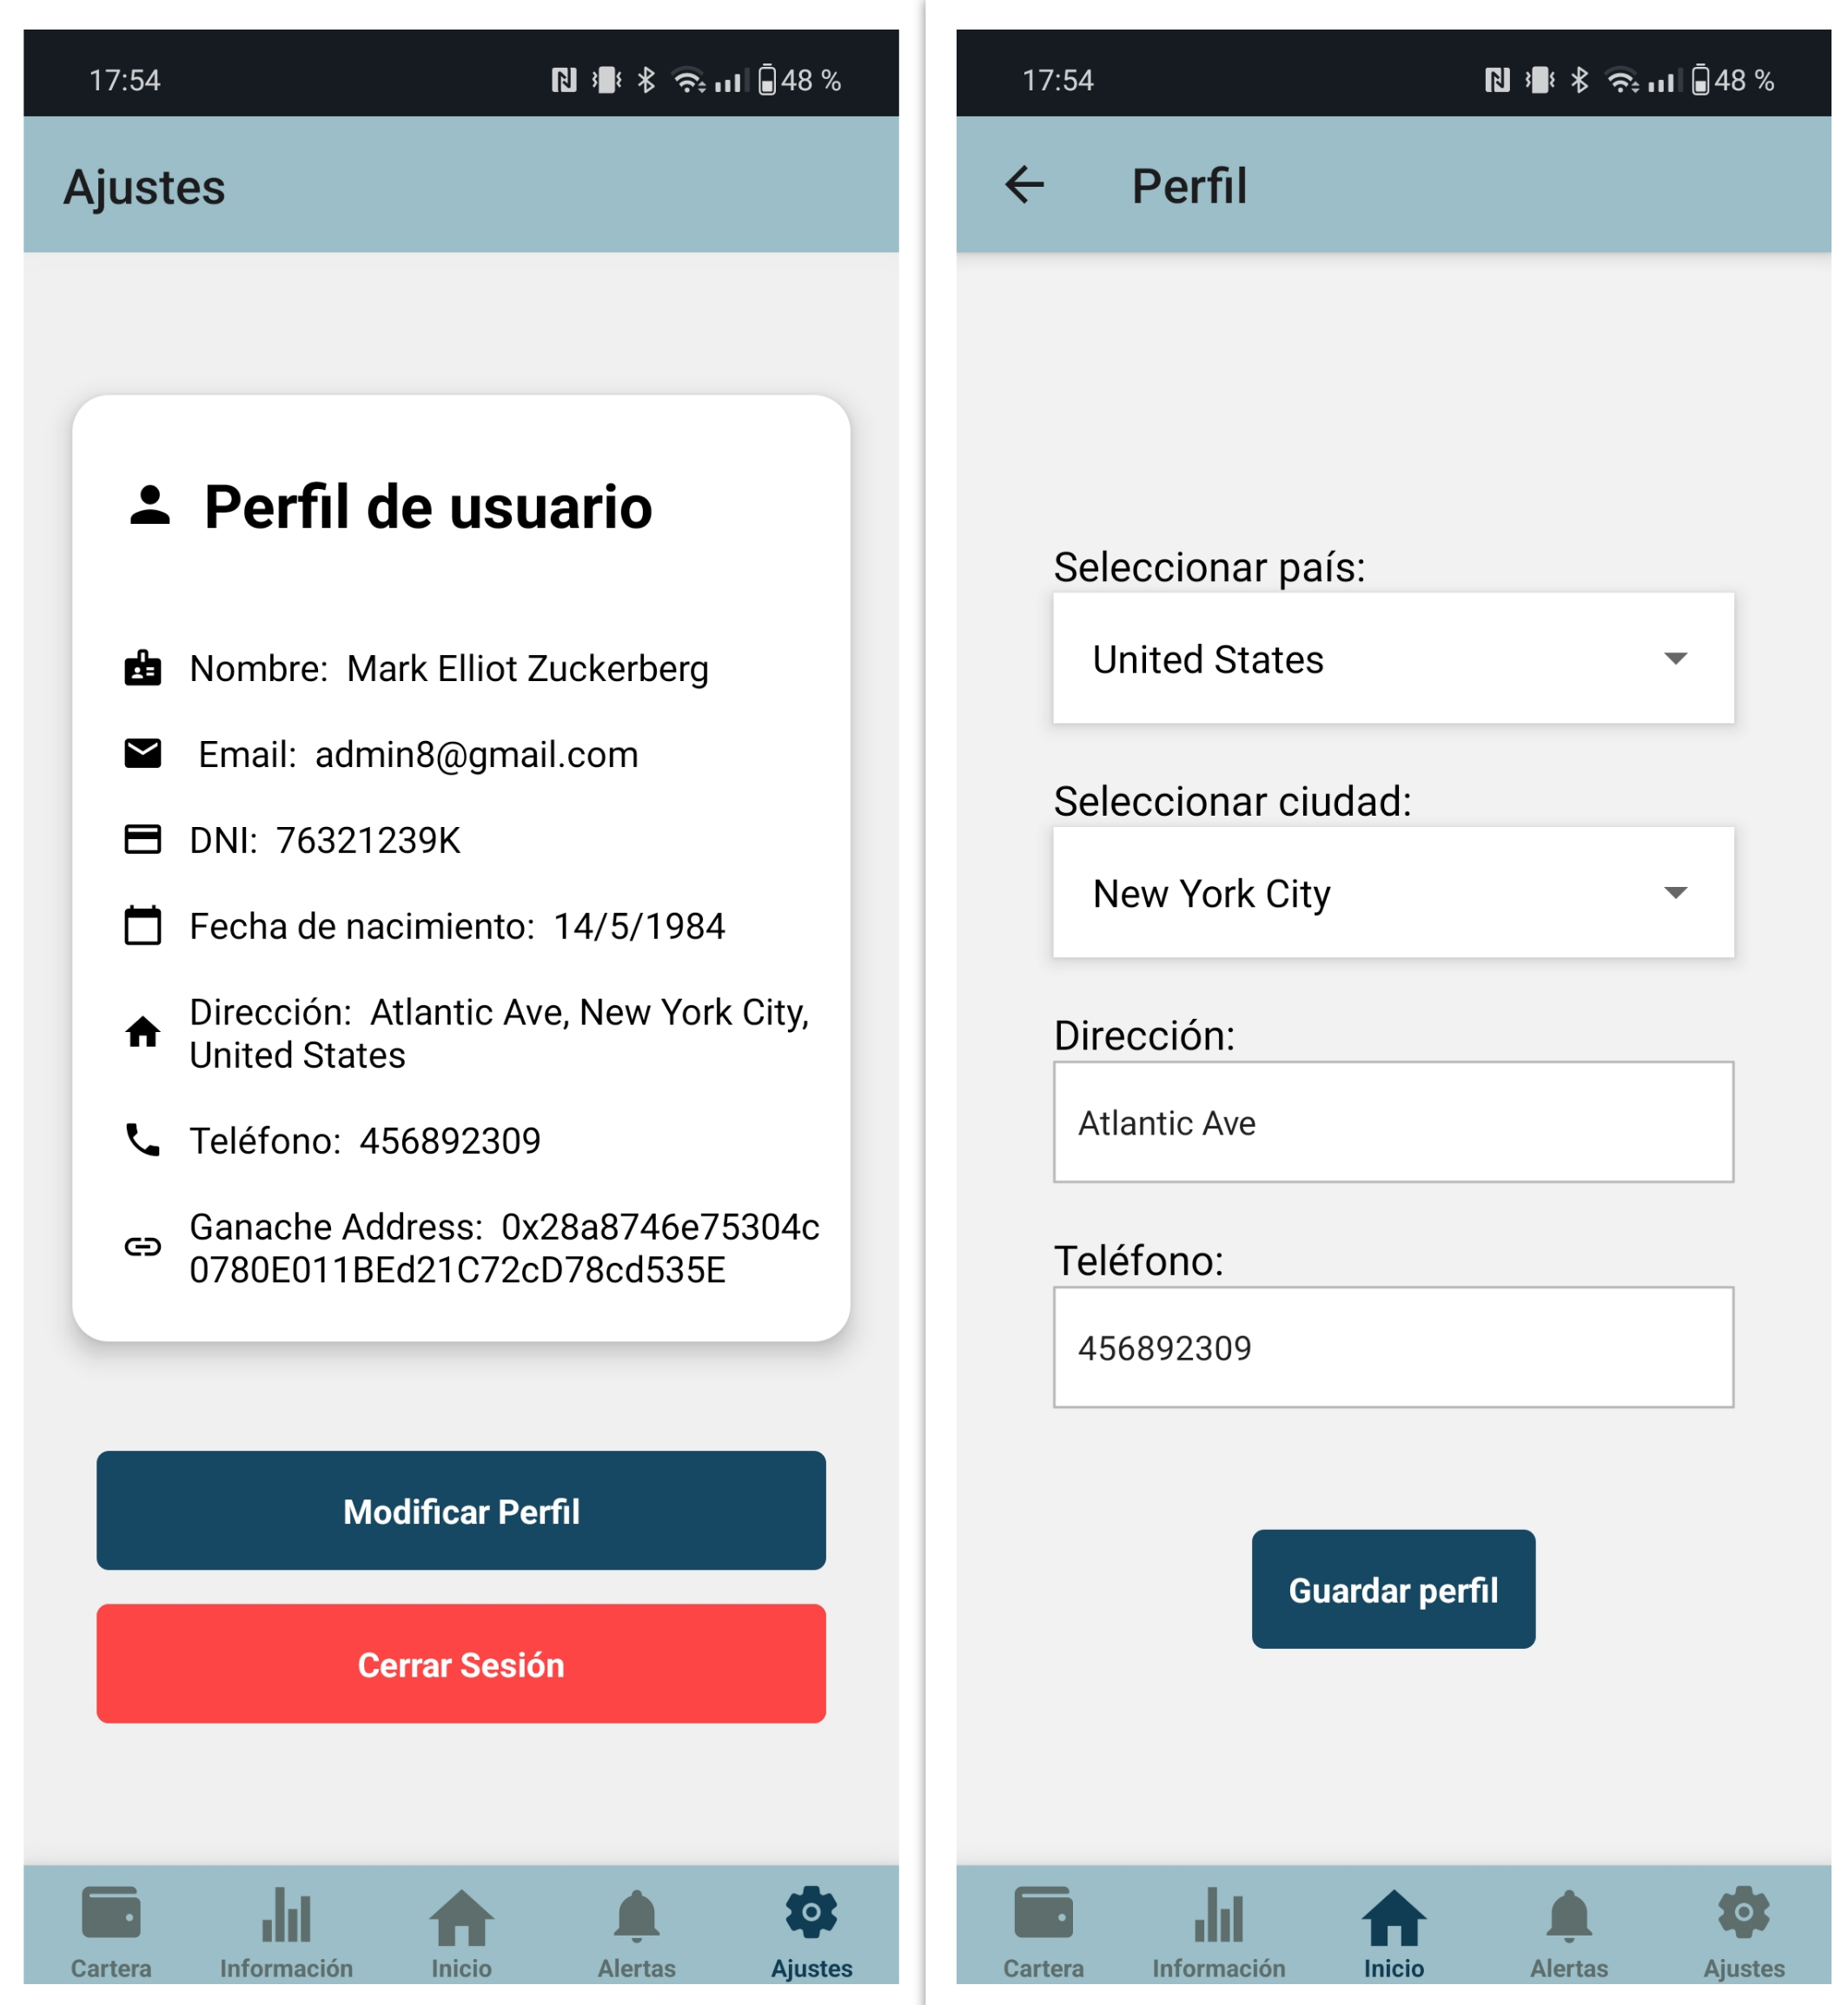
\includegraphics[width=0.90\textwidth]{perfilModificar}
	\caption[Pantallas perfil y modificación perfil]{Pantallas de visualización y modificación de perfil.}
\end{figure}



